%%%%%%%%%%%%%%%%%%%%%%%%
% Sample use of the infthesis class to prepare an MSc thesis.
% This can be used as a template to produce your own thesis.
% Date: June 2019
%
%
% The first line specifies style options for taught MSc.
% You should add a final option specifying your degree.
% *Do not* change or add any other options.
%
% So, pick one of the following:
% \documentclass[msc,deptreport,adi]{infthesis}     % Adv Design Inf
% \documentclass[msc,deptreport,ai]{infthesis}      % AI
% \documentclass[msc,deptreport,cogsci]{infthesis}  % Cognitive Sci
% \documentclass[msc,deptreport,cs]{infthesis}      % Computer Sci
% \documentclass[msc,deptreport,cyber]{infthesis}   % Cyber Sec
% \documentclass[msc,deptreport,datasci]{infthesis} % Data Sci
% \documentclass[msc,deptreport,di]{infthesis}      % Design Inf
% \documentclass[msc,deptreport,inf]{infthesis}     % Informatics
%%%%%%%%%%%%%%%%%%%%%%%%

\documentclass[mphil,deptreport,ai]{infthesis} % Do not change except to add your degree (see above).
\usepackage[final]{pdfpages}
\usepackage{siunitx}
\usepackage{hyperref}
\hypersetup{
    colorlinks=true,
    linkcolor=black,
    filecolor=gray,
    urlcolor=blue,
    pdftitle={Spiking neural network model inference},
    pdfpagemode=FullScreen,
    }

% \urlstyle{same}

\begin{document}
\begin{preliminary}

\title{Spiking neural network model construction, inference, analysis and applications}

\author{William Peer Berg}

%   Looking to machine learning and the success in applying gradient-based optimisation to tackle high-dimensional modelling problems, we here investigate the potential of applying this to the class of spiking neural network models. Further, we look at statistical assessment methods, and application of outlined methodology both to synthetically generated as well as biologically recorded in vivo data.
%   In sum, our results show that models may capture higher-order statistics of recorded nuclei, and that using some parallelisation tricks, we may decrease the computational cost to some extent. However, the lower bound on computational complexity still makes it challenging to apply the outlined methodology to very rich (i.e. high number of recorded nuclei) data sets.

% ======== Should be rewritten after main text completed. ============
% Computational models are used to try and explain observed data.
% By implementing models that replicate observed data, the model itself may explain why and how the modelled system behaves as it does, and what its function is.
% However, in order to be able to propose that the behaviour and functioning indeed arises due to mechanisms and dynamics similar to those in the model, the parallel between model properties and dynamics and in our case the brain and recorded nuclei needs to be firmly established.
% These are usually established by design, and verified by statistical comparisons over different metrics.
% However, to this day, constructing biologically interpretable and realistic models remains highly challenging, with no robust data driven approach working for other than very small networks.
% While there is significant ongoing research efforts in bridging data driven approaches with computational modelling, this remains an unsolved task for neuron-level resolution spiking neural networks with a scalable methodology.
% Currently, the most promising algorithm involves approximate Bayesian computation by training a deep neural network to approximate the posterior of the output (here spike trains) over the model parameters as the prior, and using simulation-based inference in order to generate samples, i.e. to simulate spike trains given a prior.
% As the reader may note from this, the approach does not scale well - but it does maintain a full posterior over the parameters, as they are sampled altogether.
% % SNNs biologically realistic models. 
% Do we have the tools for SNN parameter inference, instead of rigorous and tedious hand-engineering?
% ML advances: GBO.
% SNNs differ from RNNs in a fundamental/crucial way. Show via parameter landscape and loss functions.
% However, can find frontier(s).
% SNN variants and applicability of GBO (only NLIF thus far, but still local minima).
% To some extent GIF; frontier.
% Same for GLIF versions??
% Input scheme. Param landscape plots.
% Loss functions.
% PyTorch (+batching)

% ABC, (EA; e.g. NGO)

% Albeit GT off for the above, comparison wrt NMF.
% Hand-engineered case and full analysis with NMF and LDA.

% In conclusion...

% BONUS (if time): Fitting to sleep data, with small sleep regul PPT/LDT lit rev first?

% BONUS2: Append Izhikevich paper and place in context.

% BONUS3: ?


    % Neuroscience -> ML.
    % Now: ML -> Neuroscience?
    % SNNs hard. However, since DNNs work so well: SNNs as DL-case?
    % Tricks \& hacks to allow for GBO for SNNs, too!
    % Modern Pytorch-implementation - much performance, such high-level library.
    % Batching is nice.
    % Model classes. Performance over experiments with synthethic data \& GT, and on synthetic general data, and on sleep data.
    % Also probabilistic model, which lends itself better to optim by NLL, rather than frd or vrd.
    % Vrd worse probably due to stochasticity obscuring rather than refining error gradient signal w metric.
    % Param landscapes GBO
    % SBI using DNN to estimate posterior over parameters: Intractable for neuron-level (?). Compared with pop-level classes. Finding?
    
        % More data, and higher res. data available. 
    % In today's modern society, unfathomable amounts of data are generated every split second. 
     % Often experts are required to make an effort at hand-engineering models for particular data. 
        % The key ingredient to enabling this advance has been hardware-improvements, which in turn have enabled using backpropagation for large network-models, which have been shown to be universal function approximators. In other words, by scaling up the network size, one may approximate a correspondingly more complex function and data set.
    % At the very core of the inference procedure for this model class, we find gradient based optimisation (GBO).
    % In this work, I look at whether this may be leveraged for SNNs.
    % As modeling within computational neuroscience is a tedious endeavour, particularly of more biologically realistic models that entrain biological aspects in their parameters, it is natural to look at whether the successful approach for the highly complex tasks that have been solved by DL may be leveraged for SNNs.
        % , rather than the current state-of-the-art, which is simulation Based inference using approximate Bayesian computation - in fact with a DNN to estimate the posterior over the simulator (here SNN) parameters.
    % The probabilistic SNNs are compared to a published approach in which making a Bernoulli assumption over the spike history enables using the negative log likelihood for optimisation over population-level models. 
    % In this work we test all approaches for both population-level and neuron-level models.
        % NMF ensembles and geodesic dist. - spike train correlations better with SNN models than with GLMs? if not, no inductive bias / little gain with spike train as signal.
            % NLIF shows high sensitivity to initial parametrisation. also suggests ... different nature spatiotemporal signal of spike train.
    % may be fruitful to use synapse model in conjunction with the above, but overall the results suggest that under the current formulation
    
\abstract{
    Computational models have long been used as hypotheses to illuminate and unravel aspects of neural functioning, with seminal works including models such as the Hodgkin-Huxley model,
    % Models are themselves hypotheses of the system we wish to study, and may both explain functional aspects about recorded areas, and 
    which also exemplifies that model hypotheses may be tested with in vivo or vitro experiments.
    However, designing high-dimensional biologically realistic models can be an arduous endeavour, and may require hand-engineering for each setting.
    Automating this arduous process could potentially greatly accelerate computational research within neuroscience.
    Therefore, statistical approaches have been used to try and aid in such modelling, with the current state-of-the-art being based on Bayesian approximation.
    However, this approach does not scale well with growing resolution, i.e. a growing number of neurons.
    In the current data driven era, where deep learning is the prevalent state-of-the-art within machine learning, we investigate whether its key ingredient; gradient based optimisation (GBO) may be leveraged for spiking neural network (SNN) model inference.
    To this end we implement a modular gradient based optimisation framework on top of PyTorch, a modern ML Python library, and test to what extent GBO may be used for SNN inference, particularly because this approach scales well with network size.
    GBO is tested for a rate based loss metric, as well as for the van Rossum distance, which also emphasised the timing of spiking, over different classes of SNNs, including generalised versions of leaky integrate-and-fire, non-leaky integrate-and-fire, and probabilistic spiking models, with some extensions to subthreshold synaptic current models, which may enable for more continuous signals.
    The results show that due to the temporal nature of SNNs, the van Rossum distance metric and emphasis on the precise timing of spiking obscures the gradient signal due to the spike train stochasticity and resulting variability.
    Further, the parameter landscapes formed by the rate-based metric contains no saddle point, and at best a frontier as the global minima.
    These observations and results are reflected in the inferred parameters when compared to the ground-truth models for the synthetically generated data.
    As for the spike trains themselves produced by the models, we wished to test whether higher-order statistics had been captured to a greater extent yet in the SNNs, as when compared to generalised linear models as the baseline.
    When factorising the spike trains by using non-negative matrix factorisation (NMF), the resulting ensembles reveal similar functional ensembles for the synthetic data - however, the extent to which the geodesic similarity is better captured in the SNNs is very limited, and may simply be due to inductive bias.
    For the optimisation procedure itself, DNNs are known to be highly sensitive to their initial parametrisations wrt model performance and optimisation convergence.
    SNNs are no different, and seem to be even more sensitive to this, likely due to the temporal nature of the model class, in which the initial state may exert a significant effect on the modelled spike trains and futue model state.
    Overall, the results suggest that with GBO we are almost guaranteed to converge towards a local minima due to ambiguity of the loss signal, particularly when the input signal is unknown.
    Even when the input is known, such as for the sine-modulated white noise input, it is hard to correctly disentangle the signals in such a way that metrics emphasising the precise timing of spiking may be used.
    As such, it would be interesting to study closed-form non-leaky models in future work, potentially in conjunction with different synapse model, and different loss metrics that may form a better basis for gradient signal backpropagation.
}

\maketitle

\section*{Acknowledgements}

I would like to thank my supervisory team for offering their advice throughout my research.
I would also like to thank members of my lab group whom offered invaluable support and advice on everything from my project work to mastering stress and finding a flat in Edinburgh.
I also sincerely appreciated input relating to mathematics and philosophy from two special friends in Ediburgh whom are outside of my lab group - you know who you are.
Lastly, I would like to sincerely thank the head of our collaborative lab at the University of Strathclyde whom gave me access to in vivo data from the brainstem that was analysed wrt sleep regulation. It was truly inspiring and exciting to be able to see their experimental lab from early on in my project work.

% Nina.
% Matthias.
% Shuzo.
% Luke.
% Patricia.
% Etienne.

\tableofcontents
\end{preliminary}


\chapter{Introduction}


% The report then contains a bibliography and any appendices, which may go beyond
% page~40. The appendices are only for any supporting material that's important to
% go on record. However, you cannot assume markers of dissertations will read them.

% Citations (such as \cite{P1} or \cite{P2}) can be generated using
% \texttt{BibTeX}. For more advanced usage, the \texttt{natbib} package is
% recommended. You could also consider the newer \texttt{biblatex} system.

% You may not change the dissertation format (e.g., reduce the font
% size, change the margins, or reduce the line spacing from the default
% 1.5 spacing). Over length or incorrectly-formatted dissertations will
% not be accepted and you would have to modify your dissertation and
% resubmit.  You cannot assume we will check your submission before the
% final deadline and if it requires resubmission after the deadline to
% conform to the page and style requirements you will be subject to the
% usual late penalties based on your final submission time.

% MPhil:
% One who strives towards a goal to prove themselves, may suffer along the way.
% One who strives towards a goal as a means of self-expression, may enjoy the way.

\section{A synthesis from the brain to deep learning and back again?}

Spiking neural networks (SNNs) contain variables that represent biological properties such as the membrane potential, cell membrane time constant relating to the type of cell and ion channels, and potentially other neurotransmitter dynamics. Their definition results in dynamics resembling that of biological neurons, including the release of action potentials upon reaching a certain membrane potential.
Due largely to the biological plausibility of this class of neural network models, they are appealing to study in computational neuroscience, as they maintain these biological parallels, which feed-forward networks  do not.
However, SNN inference research is highly limited and faces a number of challenges due to the temporal nature of SNNs and the associated increased complexity, stemming from both state-dependence, temporal stochasticity, and parameter dimensionality.
Machine learning, with the recent surge of interest due to the large success of employing gradient based optimisation for deep neural networks, in part unlocked by the increase in available computational power and data, was originally loosely inspired by neuroscience in that we are dealing with networks of coupled nodes, thought to represent neurons.
Some of the ongoing research in computational neuroscience is now in fact focussed on whether deep learning may inspire model inference within a domain closer to its origin; namely for biologically plausible neural network models.
% This work is focussed mainly on 
We here revisit the state-of-the art for inferring SNN models using both surrogate gradient based optimisation and some of the most prominent spike metrics, as well as deep neural network amortized learning and approximate Bayesian computation (ABC), and compare how these approaches may be employed for SNN inference. Further, we hypothesise that recent ML techniques may be leveraged for successful and efficient model inference using surrogate gradient descent.
We find that while ABC may be successful for population-level models, as has been shown recently in the literature, its algorithmic and computational complexity and cost thereof limits the methodology to a low number of nodes, particularly for more high-dimensional leaky integrate-and-fire (LIF) model extensions.
However, using a surrogate gradient approach, we find that model inference for larger networks is made possible. 
Since it would greatly help with SNN model construction if automatic inference based on various data became possible and available to the research community, this has been one of my primary research goals.
Further, as usual, more and more data, and data of a higher resolution, is becoming available from neural brain recordings, only increasing the potential benefits of developing a scalable approach for model inference.
We perform model inference using a set of LIF-extensions, leading up to the GLIF model using (both) synthetic (and biological) data, and demonstrate that higher order statistics may be captured (to some extent) even when performing neuron-level model inference over a mixed neuron-type network.
% This may advance research on SNN inference, and also demonstrates how modern ML frameworks as well as techniques may be leveraged to this end.
However, we observe that it is highly problematic to aim for retrieving ground-truth parameters in SNN models. A large part of the work presented in this thesis will revolve around why SNNs do not lend themselves as well as feedforward neural networks as within deep learning, even though they also implement a type of recurrence using recurrent units with memory, in addition to potential recurrent connectedness.
To try and give an intuition about why this is; if we think about deep neural networks (DNNs) in the machine learning (ML) domain - these may approximate arbitrary data well, given that they are universal function approximators. However, this requires that the data is of such a format that it may be represented and captured by a function which the network learns by spatial representation and transformation.
However, in the domain of SNNs, we introduce several new crucial properties, which results in distinct model dynamics. Each neuron now has a state, which depends on its previous state, and the behaviour is modelled typically as a system of ordinary differential equations (ODEs), containing parameters representing the membrane potential, membrane time constant relating to a refractory period, transmitter interaction, and other biological properties. 
While this makes the model biologically interpretable with direct parallels between parameters and biological and cellular counterparts, it also changes the entire system's behaviour.
The system now has activity inedpendently of input perturbation. The transformation of an input signal is no longer deterministic in the sense that it will result in one given output given a set of initial model parameters - it now depends on the current system's state, which again depends on the previous state.
As such, gradients calculated in a manner similar to that of for DNNs in ML will also depend on the system's and neurons' state, greatly increasing complexity.
In a way, one may still maintain the parallel to backpropagation through time for DNNs - however, there is a crucial difference in that a neuron's output is now of a much more binary nature; a spike or no spike, and in that the time series evolution of spikes, whilst potentially encoding much more information, now is a series of spike evolving over time, and thus the target signal cannot be regarded in the same way as in DNNs.
This being said, I believe like noted by other authors such as \cite{Sindaci2018} that researchers are looking for a connection between the field of machine learning and computational neuroscience, the former having had its subfield of DNNs created based on inspiration from the brain, but now in a reverse way in which we may leverage the advances from the domain of ML in model construction.
Even though we are not there yet, I believe the search for a connection here may both be highly beneficial for the community, and spawn a new sub-field of dynamical systems modelling using inference in computational neuroscience.

% My main findings, although included throughout in the rest of my thesis, may be summarised as following:
Although SNN inference certainly would be of great value to the field, there are some key issues that I have identified and tried to address in my work, some of which are included in the subsections below.

\section{SNNs are hard to optimise}
% I am starting to believe that they’re in fact not possible to optimise, due to the parameter landscape, which results from the temporal nature of the target signal.
In DNNs, we only consider approximating a spatial transformation over the input data. Not only does this allow for higher parallelisation of the training algorithm, but it may also greatly constrain the parameter landscape in the sense that it does not depend on the past activity of the network itself, which vastly increases both the complexity and stochasticity of parameter inference. 
One way to ameliorate this is to eliminate some of the stochasticity by making the neurons non-leaky. Since we may computationally set the system’s initial conditions and random seed, the following deterministic computations have little to no fluctuations, and with no leakage, gradient propagation may be computed exactly according to the error signal.

However, there should exist solutions to the set of coupled ODEs that maximise a given loss metric. The question would then be how large the solution space is, and to what extent the different regions are reachable. Furthermore, we are not guaranteed that the solution(s) given by our metric captures the precise temporal dynamics. In fact, it is limited how much of this information can be incorporated into and made relevant by the loss metric.
Nevertheless, since BPTT and optimisation for DNNs within DL has been shown to be able to be able to infer highly complex data sets, it is our goal to study the extent to which a similar methodology may be applied in SNNs, to evaluate the performance of this novel algorithmic design, and to illuminate where work that bears potential may lie.


\section{The binary nature of spiking}
One way of addressing this issue is by incorporating the signal below spike-threshold, i.e. the membrane potential, and have this generate a signal inside of an active zone, such as when the potential is above 0. This is not entirely biologically unrealistic, …, and it offers the advantage of a continuous signal centred around potential (no pun intended) spike pulses, or action potentials. Note that it also provides a gradient signal for spike generation even when the potential may be below threshold, still making the excitation visible to the optimiser.
This bears some resemblance to loss metrics such as the van Rossum distance, in which each spike pulse is convolved with an exponentially decaying kernel, such that we may operate over a smoother signal. However, this signal transformation transforms each spike pulse the same, rendering the sub-threshold gating synapse model a more fine-grained candidate, since it contains richer differentiable information, and not just spike-time information.

Temporal kernel no new information - but transforms signal such that it contains a trace which may be more easily optimised. Think about aligning two waveforms, rather than two short pulses, where the information gain is only visible in the step which matches them.


\section{The parameter landscape contains a frontier with local minima}
Even when addressing the issues above with the proposed approaches, and even if fixing all model parameters but the weight matrices, there are multiple weight configurations that may result in very similar behaviour and outputs.
As noted by other researchers in the DNN as well as SNN literature (...) the initial configuration has a large effect on the resulting inferred weights and/or model. This holds particularly true for SNNs, where the previous model state also has an effect on the future state, and the model neurons may be brought to exert different modes of behaviour, depending on the previous and current input and state.

\section{Hand-engineered models may be qualitatively similar to local minima}
By hand-engineering models it is possible to attain qualitative patterns and behaviour, which has been a common practice in the field of comp neuro - however, this may not be satisfactory for attaining higher-order statistics, and requires a large amount of resources. Therefore, model inference may likely be a better option. 
The above however indicates that GLMs may be the best we can do in this regard (wrt spike trains), and demonstrates a need for advancing SNN inference.
The way going forward?
Amortised learning provides a posterior over the parameters.
However, it quickly becomes intractable due to the high complexity of models.
Surrogate or exact gradient approaches are difficult due to aforementioned issues, and most likely do not settle into a stable configuration, as well as stay in planes of local minima.
These findings suggest that the best we can currently do is using approximate Bayesian approaches, which not only lets us infer a posterior over all of the parameters, but also provides a measure of certainty around the parameters.

\section{Temmporary conclusion}
If this approach is intractable for the case we’re looking at, the best we may do is either to use other information theoretic approaches to assess whichever aspect it is that we are interested in, including potentially to hand-engineer and rigorously test a proposed model.


% =======================================================
% =======================================================
\chapter{Background: Biologically plausible computational modeling}

% Mainly surrogate gradient descent, but also some conversion approaches.
Learning in SNNs; multiple model definitions and topologies, affecting the way in which learning may be performed - from perceptron to HH, from single-neuron to multilayer.
HH complex enough that fitting the parameters of a single node using electrophysiological data requires a significant amount of computational resources.
% The \cite{HH1952} 1952 paper more or less hand designing the ODE system in a way that generalises well to describe neuronal and cellular electrophysiology.
Perceptrons highly implausible.

Supervised, semi-supervised - different tasks.

There are different approaches for tackling the different nature of SNNs. 
On the one hand the temporal unfolding of the internal state and their significantly exerted effect on activity requires loss metrics that are adopted to also measure this effect, and on the other limited information when modeling biological data poses a constraint on the extent to which timing may be emphasised.
Further, the explicit encoding scheme adapted in SNNs is traditionally a type of rate-based encoding - but this does not make use of the rich information available in the timing of spiking.
Population-encoding is another type of approach which may make readouts and learning more stable in a network, but also imposes a significant information bottleneck on the amount of information that may be processed and encoded by the network.
It is likely that the brain employs an encoding scheme in which the rich information contained in the timing of spikes is relevant - however, principles in which these may be learned are non-trivial to devise, or are non-applicable to noisy data with unkown input.
% TODO: Update. Also make scope and goal of modeling bio. data much clearer! (gjennomsyre tekst)

% Various SNN models
\cite{Taherkhani2020} learning in SNNs

% Mackelab meso paper: Only rate based at first.
% NN 2020 review: Loses out on temporal information.
% NMF: Spatiotemporal decomposition - thus rate based should not be able to infer spatial activation coefficients. However, encode populations into SGD, and rate based may? 
% Topological averaging.
% Search using micro-model directly? Data set requirements? Spike trains - rate per node and binom dist.?


\section{Fundamental differences between SNNs and spike train PDF models}

A spike train can be modeled by drawing from a probability distribution $P(X; \lambda)$.
This is perhaps the simplest baseline model one may construct, also assuming complete independence between neurons in a data set.
However, this type of model may quickly break down when not assuming dependence between neurons.
It may also be updated assuming independence, resulting in a more complex PDF.
A more robust baseline model would be a generalised linear model, in which ... Poisson PDF and coupled nodes.
This may capture spike correlations and rates better, but not exert different modes of behaviour.
I.e. it is a spatiotemporal model with fixed temporal signatures which may be slightly affected by input, but not fundamentally change its dynamics and behaviour, as opposed to in SNNs.
The golden goal should as such be to infer models that capture the different modes of behaviour, thus also the dynamics that are at play and may be exerted under different input conditions.
This may be extremely hard to capture using current inference methodologies, and has to the best of my knowledge not been successfully attained by the research community.
(...)
It is something that may be tested by designing different input conditions for a model synthetically - and also tested in vitro or vivo by stimulation e.g. optogenetically or using more traditional patch-clamp tissue stimulation.

Typical leaky integrate-and-fire SNN neuron model definition:

\begin{equation}
    \tau_m \frac{dv}{dt} = E_L - v(t) + I(t)
\end{equation}

where $v(t)$ is the membrane potential, and $I(t)$ is the synaptic current, usually summing over some stimulus as well as neuronal synaptic inputs and associated weights, potentially summed through a transfer function that bounds the current,

\begin{equation}
    I = \sum_{i,j}^{N} W_{i,j} s_i + I_{ext}
\end{equation}

where $W_{i,j}$ is the synaptic weight from neuron $i$ to neuron $j$, and $s_i$ is the pre-synaptic current from neuron $i$.

\section{The link to recurrent neural networks (RNNs)}

As mentioned previously, SNNs are systems in which each node is a set of ODEs, where each variable or parameter may have a more or less direct biological parallel, such as representing the rest potential $E_L$, the spike threshold $V$, and other properties.
Together, these result in a model whose membrane potential $v_t$ has a temporal trajectory similar to that of biological neurons.
The main idea is that under the right conditions, these models may mimic biology so closely, that we can in fact use them to study what might be going on in a brain area, where the model is the hypothesis.
The stronger the link between the model and the brain area, the stronger the hypothesis, and predictions based upon probing model dynamics under various conditions.

In RNNs, however, the criterion of each node or neuron being a system of ODEs that maintain biological parallels is relaxed. Each node may simply be one value that is some sum over synaptic input that has been transformed by a transfer function, or it is more commonly some slightly more complex units such as gated recurrent units (GRUs) \cite{Bengio2013b, Chung2015a} or long short-term memory units (LSTMs) in machine learning \cite{Hochreiter1997, Schmidhuber2014}.
If dealing with nodes as common in machine learning, the temporal dependence is more limited than in more complex SNNs and neuronal ODE systems.
Further, RNNs are usually trained on tasks in which the input is known, and is some static "spatial" transformation of inputs to outputs, which forms the data set.
In other words, the data to be modeled is usually non-noisy, and of a more straightforward nature than (decoded) brain recordings such as spike trains.
These aspects make the models far more suitable for chaining the error gradients backwards in time, which may be done over each time-step for each error gradient by a modification to the backprop-algorithm, known as back-propagation through time (BPTT).
Note also that RNNs typically deal with continuous, smooth signals in each node, whereas SNNs traditionally and usually function more as perceptrons in that their activity is binary, which also complicates training, let alone inference of model parameters other than the weights.
Typically, only the weights are inferred in ML using some gradient based optimisation algorithm.
There exists, however, work in which SNNs are transformed such that they are more compatible with BPTT, including probabilistic models in which each node projects a probability of spiking for each time step or interval, and models in which synaptic signals are made continuous and smooth, either by constructing a surrogate over the membrane potential, or by modeling the signals as a function over the subthreshold membrane potential, such as for instance when it is above zero, or within a given interval, resulting in a synaptic current.
% The former approach has been studied in works such as \cite{}
\cite{Neftci2019} describe the connection between RNNs and SNNs well, including the efforts that have been made to employ (surrogate) gradient descent for spiking neural networks.
% Should talk about points relating to where rate-based metrics is the best one can do wrt spikes

When working with spike probability based SNNs there is model stochasticity that render precise spike timing based metrics worse than rate based metrics, as the timing is no longer meaningful, and only obscures the gradient.

The same often holds for SNNs in which surrogates are constructed, due to elements such as the initial model configuration, initial conditions, or model perturbation.
Works such as \cite{Jin2018} employ a rate-based error metric for data and readouts pertaining to image classification tasks.
By considering how these complex systems behave differently under different conditions, and that they may be heavily affected by their current and thus past state, approaches pertaining to rate codes seem to be the extent to which many works are able to incorporate temporal precision and successfully optimise the models.
While these works are valuable in studying how one might combine optimisation and spiking models, they often are limited to not only rate-based encodings and/or loss metrics, but also to non-noisy ML domain types of data.
However, the sole basis for studying SNNs in computational neuriscience is to maintain the biological parallel, such that the model may be used as an interpretable system and hypothesis of recorded site dynamics, and studied as such.
Therefore, it is important to study how the precise timing of spiking may be made relevant in the models, as that is arguably not only a relevant source of information, but a rich encoding scheme employed by the neural circuitry in the biological brain.
While this was initially debated, it has been argued both by information theorists, neuroscientists and computer scientists alike recently that the precise timing of spiking is not only relevant, but is in fact necessary in order to encode all of the information that has shown to be processed by the brain, i.e. a rate-coding is not enough to represent a task which is solved by a neural network.
% references

% RNN transfer function, unit as GRU versus dv/dt etc.
\begin{math}
    \textbf{h}_t^j = \textit{f}(W^{i,j}\textbf{h}_t^i) + \sum_{i=1}^L g^{i,j} U^{i,j}\textbf{h}_{t-1}^i
\end{math}

in essence

\begin{math}
    g^{i,j} = \sigma ( \textbf{w}_g^{i,j}\textbf{h}_t^{i} + \textbf{u}_g^{i,j}\textbf{h}_{t-1}^{*})
\end{math}

basically treating the network instead of a conventional RNN which may be regarded as a POMDP process as a process in which each hidden layer has gated recurrent connections determined by a reset gate function, which allows the ignoring of previous hidden states by transition through the reset gate function, whose weights may also be updated by the same methodology;
estimating a probability distribution over sequences, factorising the probability of the sequences, and training an RNN by means of negative log-likelihood minimisation of the training sequences:

\begin{math}
    p(x_1, ..., x_N) = p(x_1)p(x_2|x_1) ... p(x_N|x_1,...,x_{N-1}), \\
    p(x_N|x_1,...,x_{N-1}) = g(\textbf{h}_t)
\end{math}

Note that this bears resemblance to SNNs, and is bridged particularly by the probabilistic model version of \cite{Rene2020}, which we have based a spike time and gradient compatible model implementation on in section \ref{microGIF}.
There, a spike train is assumed to be a Bernoulli distributed spike history, which may be estimated with the ODE system and its recurrent connections.
However, connections are there optimised in a more straightforward manner, with the other parameters and internal dynamics instead being what decides on the "gating".

In my work I have studied employing gradient based optimisation as well as approximate Bayesian computation using amortised learning for both a probabilistic class of stochastic spiking neural networks \cite{Rene2020}, for leaky types of integrate-and-fire SNNs \cite{allen_glif_white_paper}, and for closed-form (still with multiple solutions?) exact-gradient types of non-leaky integrate-and-fire SNNs \cite{Huh2017}.
I have also replicated and analysed Izhikevich SNNs, but chosen not to apply GBO to this model class due to planes of chaos in the parameter landscape, simply resulting in that the Izhikevich neuron ODEs are a lower-dimensional projection of the Hodgkin-Huxley ODEs - resulting in that while they are of lower complexity simulation-wise, the collapse of several variables into fewer results in variable intervals for which model behaviour is unrealistic and/or chaotic, making GBO impossible.


\section{Bayesian approaches}

Sample of observations O given priors p, Bayes rule; posterior over parameters given observation, i.e. data.

\begin{equation}
    P(\theta|X_o) = \frac{P(x_o|\theta)P(x_o)}{P(\theta)}
\end{equation}

One way of going about this is to generate observations with a simulator, for which we may generate samples over priors, enabling us to estimate a full posterior over the parameters for a given observation.
Note that this does not omit the difficulty of model conditions, including model perturbation and external input.
Further, the computational cost requires sampling a great number of samples in order to estimate the posterior over the parameters, thus increasing drastically with the model dimensionality and number of parameters.
The approach does, however, come with the benefit of being able to assess and directly measure the certainty by usual statistical metrics around the centres of the posterior distributions, as well as that the full posterior distribution contains samples across all parameters, dependently, which may capture dependencies not so easily captured when estimating using GBO.

\subsection{MCMC sampling}
\cite{Rene2020} "special case" i.e. mesoscopic-microscopic inference using first ABC (or GD?) on pop. level and then MCMC sampling for full approx. posterior?

“To understand how rich dynamics emerge in neural populations, we require models which exhibit a wide range of dynamics while remaining interpretable in terms of con- nectivity and single-neuron dynamics. However, it has been challenging to fit such mechanistic spiking networks at the single neuron scale to empirical population data. To close this gap, we propose to fit such data at a meso scale, using a mechanistic but low-dimensional and hence statistically tractable model.”
Argue that instead of making the reduction to a population-level model, we may instead make the dimensionality reduction for the parameters.
There exists work on fitting GLIF parameters to physiological data. 
Also, inferring weights with fixed parameters is possible using GD, given data.
This could mean that we could, given the correct neuron classes, infer a topology or the connectivity of a site recorded from!
Parameters may be inferred prior to the weights using an appropriate procedure.
However, in the Rene-paper they use aggregate population activity, or spike histories, and derive the likelihood for the parameters. Can be used to either optimise, or do Bayesian inference.
They conclude that population inference impact and improve the accuracy in single-neuron parameter inference.

The René paper assumed known input when inferring models. They also generated data with sine-modulated input.
They also made a quasi-renewal approximation, and assumed independence between neurons in each time bin.


\subsection{Amortised learning with DNNs}

% SNPE
\cite{Lueckmann2018} amortised learning and ABC using DNNs.

Since DNNs are universal function approximators, they may be used to approximate the function of the posterior distribution over the parameters given observations for a given model system.
It seems that DL is an excellent candidate for this type of function approximation, and that in this regard GBO works just as well as it does in ML, depending on how well-defined the posterior distribution in fact is in the data.
We find in our work that particularly when working with models that have larger spaces which I like to think of as "frontiers" in the parameter landscape for which the loss is approximately equal, the posterior is similarly not condensed around fixed points.
\cite{Lueckmann2021} (double check ref.) however find that the posterior approximation still contains the relationship, i.e. dependence, over the parameters. 
In other words, while they cannot be sampled independently for marginals, sampling over the full posterior still generates realistic data.

% The good old Bayes' rule:
% \begin{math}
%     P(\theta|X_o) = \frac{P(x_o|\theta)P(x_o)}{P(\theta)}
% \end{math}

\begin{math}
    O: \Phi(\theta) \sim X, \quad
    DNN = F_\Phi(\theta; X) \approx P(\theta|X)
\end{math}

There usually is a larger space for which performance given by the loss metric is fairly equal, just requiring a different combination of parameters - i.e. there is no single fixed point or trajectory leading to it in the parameter landscape leading to a global minimum.
My interpretation of this is that what we identify with learning algorithms for SNNs is not a specific configuration which captures the data set at hand, but a configuration which reaches a mode of behaviour that would allow it do produce the data.
This may indicate that there are other principles underlying the learning of these networks.

% \section{(Evolutionary algorithms)}
% \section{Gradient free optimisation with evolutionary algorithms}

% I recall back to conferences talking about inferring complex, deep networks, which is a field where evolutionary algorithms (EAs) still are competitive and fruitful.
% In short, when EAs are fruitful, this often means the search space is so vast that gradient-based approaches will not converge.
% Even so, the computational cost is comparable, or even worse, than for ABC.

% NGO

% let's forget about casting the spike trains into a euclidean space, and propagating gradients. let's relax this to defined operations where there is a cost assigned to each operation, such that there is a minimal distance between two spike trains. this should let us define operations for moving single spikes, and shifting spikes. however, in my case there is uncertainty involved, so we should define operations for matching motifs instead. this makes it unclear for polynomial-time DP for calculating the distance. i can do pattern identification according to pre-defined rules, which will be exponential over a constant bound such that for longer time-intervals, a greedy comparison should be polynomial.
% if we assume that parts cannot cross in graph-matching, however, it becomes polynomial for the full distance-calculation (for larger intervals)

% sin (f(s)) + cos (g(s)) ?
% where f(s) = D\^spike[q, k]
% and g(s) = D\^interval[q, k]
% assume same labels?
% --> However, does not converge well.

% nevergrad + brian2
% for efficiency purposes..?
% Evolutionary algorithms may be used to traverse high-dimensional parameter-spaces in search for optimal solutions to complex problems such as fitting complex network models.
% This is made possible by by using objective functions to evaluate solution candidates, essentially provided as heuristics guiding the search. Note that finding the global optimum cannot be guaranteed when using evolutionary algorithms.
% In our case, due to the nature of the GLIF model, we may both constrain the parameter search space to meaningful parameter intervals, and employ search strategies that are more suited for the system.

% Two such evolutionary algorithm strategies are differential evolution (DE), and covariance matrix adaptation (CMA). 

% By using differential evolution (DE), a strategy where a set of best performing candidates are combined and mutated, we may continuously improve parts of the candidate solution, whilst potentially naturally constraining the search as a result.
% % revise the above
% While DE may be used to cross over and generate candidate solutions more broadly, it may also be skewed towards local optima. Another approach that we selected that might be better suited for very high-dimensional problems, is covariance matrix adaptation (CMA) evolution \cite{Igel2007}. CMA will naturally utilise correlated parameters in the model system as is the case in the GLIF model, and incorporates this by updating a covariance matrix during search path traversal, which is in turn used to maximise the probability for finding successful candidate solutions.
% Effectively, CMA does principal components analysis over its evolution path, which allows for variance and step size adjustment.
% CMA evolutionary strategies have been shown to perform well for difficult functions with larger budgets \cite{Hansen2010}.
% % revise the above

% % PSO, NGO?
% Initial testing with particle-swarm optimisation (PSO), which can be said to search more widely before converging towards the best performing candidate in the fitness landscape.
% However, divergence or non-converging bad fits, likely due to the vast complexity of the parameter-space and the nature of PSO.
% Failure to converge to results of comparable loss to the other optimisers was also the case with neighbourhood and genetic operator (NGO) search.



\section{Evaluating SNN models}

% Not straightforward how to analyse... 
% Should this be in background or later?
Refer reader to report or poster in which these are explained, and only provide "glue"-text here, explaining usage and placing them in the context?
\cite{Seung1999, Seung2001, Onken2016a}

\subsection{NMF}

In order to assess functional organization in the neural data we employ non-negative matrix factorization (NMF) \cite{Seung1999} to infer ensembles of coactive neurons. 
% NMF is a dimensionality reduction technique which has been shown to be particularly suitable and well-performing for neural data \cite{Onken2016a}.
This factorization may be written as,

\begin{equation}
    M \approx WH,
\end{equation}

where the original data set $V$ of dimension $n \times t$ is factorised into two matrices of dimensionality $m \times n$ and $m \times t$.
What makes this dimensionality reduction method particularly suited for spike train data is its non-negativity constraint, which naturally leads to a parts-based representation. % Further, NMF has been shown to outperform other common dimensionality reductions such as independent component analysis, principal component analysis, and factor analysis \cite{Onken2016a}.

While NMF may be used to discover spatial and temporal firing patterns in spike data, the geodesic similarity measure between the modules may be used to assess how well these features were recovered in a fitted model.
The geodesic distance $o$ between two matrices $A$ and $B$ of dimensionality $m \times n$ may be written as,

\begin{equation}
    o(A, B) = (1-\frac{2}{\pi}\cos^{-1}(A^TB)),
\end{equation}

where $m$ is the number of modules, and $n$ is the number of nodes in the data set. 

\subsection{LDA}

% linreg for separating hyperplane with arbitrary kernel? or simply linear transformations?
% \subsection{Random forest}
\cite{Onken2016a}


\subsection{Baseline: Generalised Linear Models}

\cite{Nelder1972, Fernandez2000}

Spike counts assumed to be Poisson distributed, and may thus be approximated by a Poisson PDF,

\begin{equation}
    y_t|x_t, w \sim Poiss(y_t; f(x_t^T w)\Delta)
\end{equation}

this gives the log-likelihood of

\begin{equation}
    log p(y|X, w) = \sum_{t=1}^T log p(y_t| x_t, w) = \sum_{t=1}^T(y_t log f(x_t^Tw) - f(x_t^Tw)\Delta)
\end{equation}

which may be approximated using MAP estimates by numerical methods.
Further, coupled GLMs, in which spike histories depend on one another, may also be approximated. This allows to capture second-order and potentially higher-order spike correlations, depending on the link functions used.

GLMs are a suitable basline model for spike train data, as spike trains are Poissonian in nature, and thus fitting parameters for a Poisson probability distribution for each node provides spike trains of similar nature.
Further, to capture correlations between neurons in spike trains, this definition may be expanded over a set of probability distributions, where each is parameter is dependent on the others.

For more details, please see the references included above, or the sample code given in \ref{appendix:sample_GLM_code}.

% TODO: Consider expanding a bit wrt model definition and inference.


\section{Model definitions}

\begin{figure}
    \centering
    \vskip -0.1in
    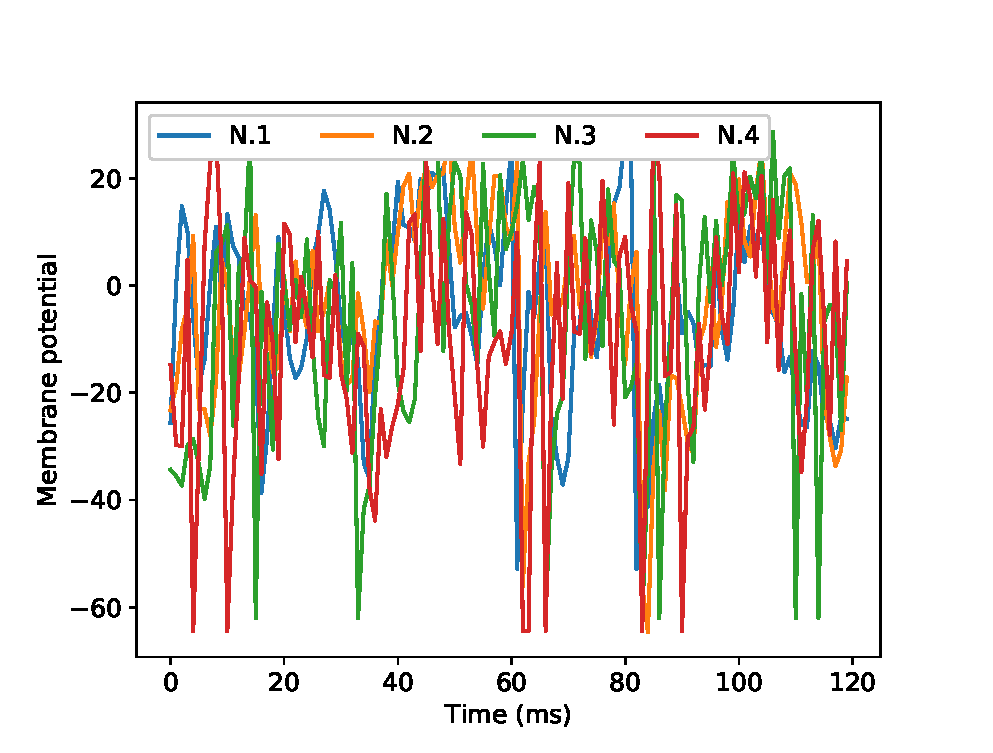
\includegraphics[width=0.33\columnwidth]{figures/samples/membrane_potentials/export_sample_LIF_white_noise.eps}
    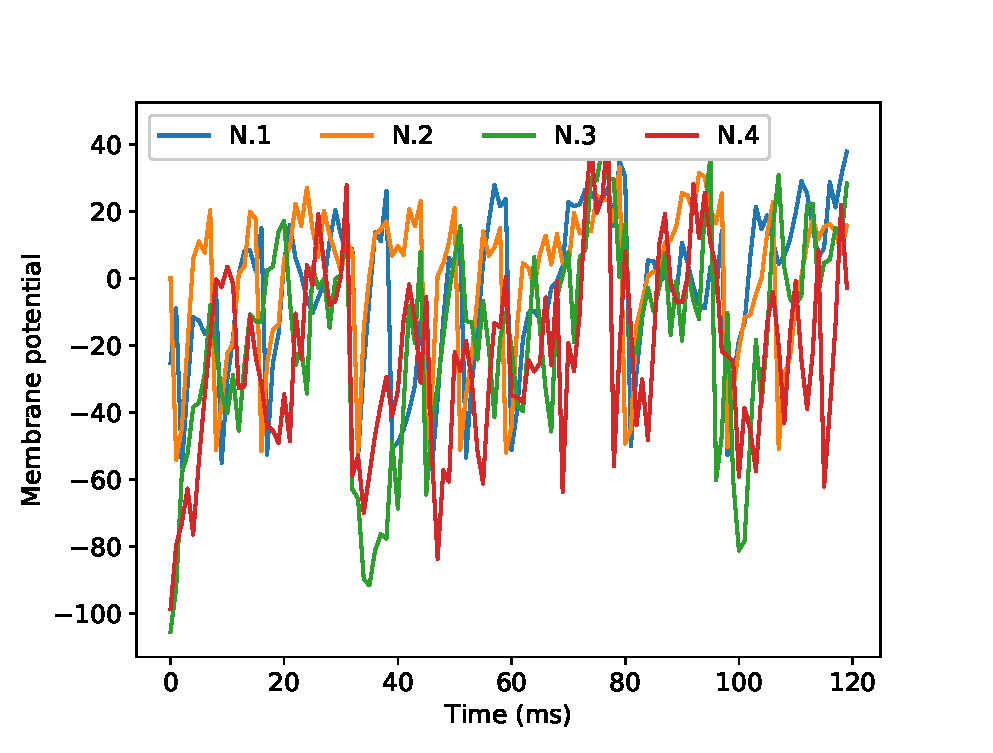
\includegraphics[width=0.33\columnwidth]{figures/samples/membrane_potentials/export_sample_GLIF_white_noise.eps}
    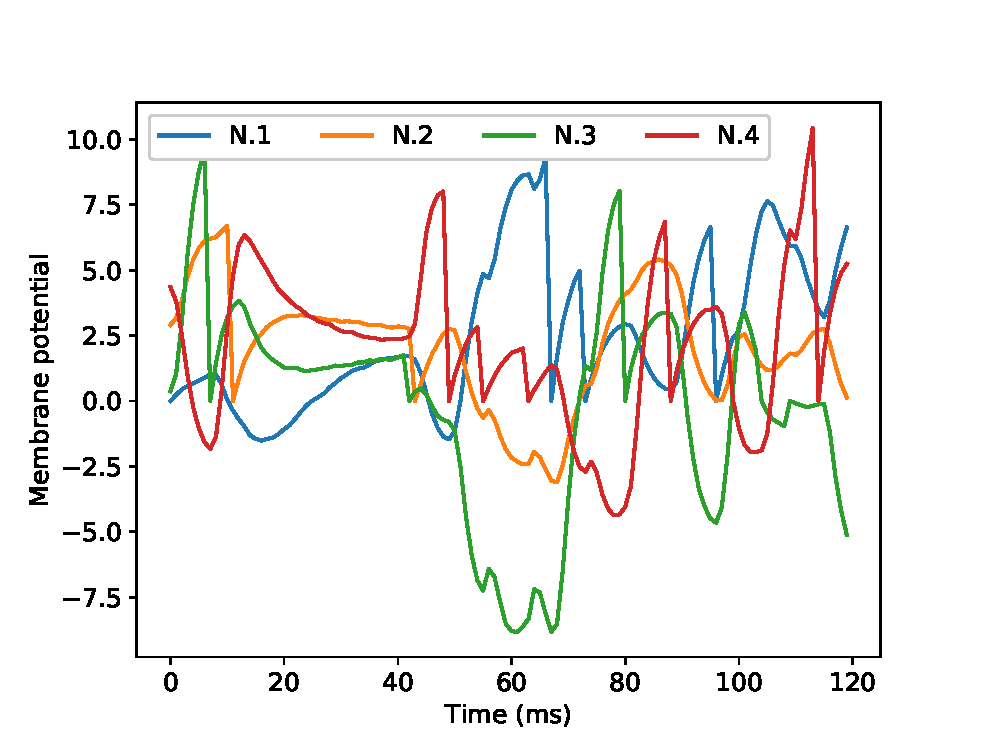
\includegraphics[width=0.33\columnwidth]{figures/samples/membrane_potentials/export_sample_mesoGIF_white_noise.eps}
    \vskip -0.1in
    \caption{membrane potential samples}
    \label{fig:membrane_potential_samples}
    \vskip -0.2in
\end{figure}

\subsection{LIF}

% Write out definition, discuss a bit..? Refer to paper.
Included portion of paper:

The neuron model we employed in this work is the leaky integrate-and-fire (LIF) model, as described in among other works \cite{Rolls1998Book},

\begin{equation}
    \frac{dv}{dt} = \frac{E_L - v_t + R_I I_t}{\tau_m},
\end{equation}

where $E_L$ is the rest potential, $v_t$ is the membrane potential at time $t$, $R_I$ is the membrane resistance, and $I_t$ is the synaptic current.
The modelled networks are non-transitively fully connected, with the weights normally distributed between $w \in [-1, 1]$. The synapses are modelled as exponentially decaying post-synaptic currents, where a conductance variable $g$ models the conductance for the neurons,

\begin{equation}
    \frac{dg}{dt} = -\frac{g}{\tau_g},
\end{equation}

where the synaptic input current to a neuron $j$ is modelled as $I_{syn,j} = \sum_{i} w_{i,j} I_{i,j}$.

While forward passes are done according to a spike-threshold function with non-linear resetting of the membrane potential upon spiking, the backward pass is made possible by separately defining a differentiable soft-threshold function over the membrane potential which is used solely for back-propagating the error gradients obtained by minimizing the loss functions. We use the commonly applied sigmoidal function for this purpose,

\begin{equation}
    s_t(v) = \frac{1}{1+e^{-(v_t))}},
\end{equation}

where $s_t$ denotes whether a neuron spikes at time $t$ with a membrane potential $v_t$.
This results in that optimization of defined loss metrics always back-propagates error gradients through the soft-thresholded membrane potential, in effect treating this as a continuous spike value. 
In other words, the distance metrics calculate the distance between a continuous spike train to a binary target spike train.
Note that this also results in that sub-threshold values result in a spike signal during optimization.

% TODO: Update.
% \begin{figure}
%     \centering
%     \vskip -0.1in
%     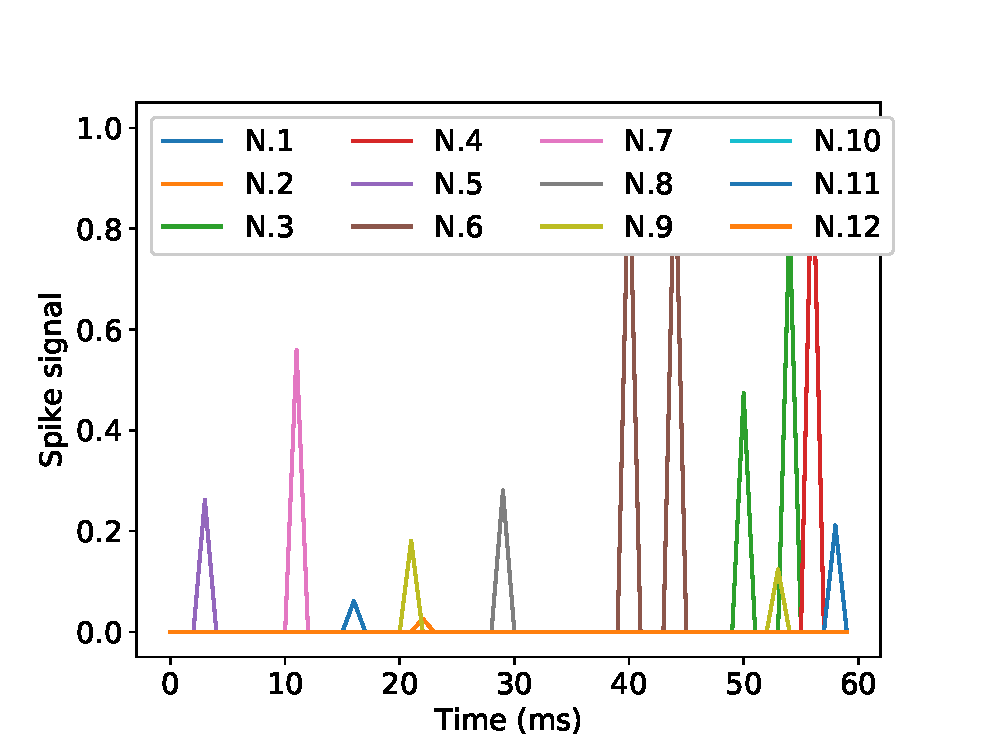
\includegraphics[width=0.9\columnwidth]{figures/plot_spike_thresh_lif_ensembles_dales_0.eps}
%     \vskip -0.1in
%     \caption{The soft-thresholded spike signal $s_t(v)$ for $60 \si{\ms}$ backward passes during model simulation for $12$ neurons.}
%     \label{fig:spike_thresh}
%     \vskip -0.2in
% \end{figure}

All parameters were held as free parameters during optimization, resulting in 4 $N$-dimensional free parameters, and one $N^2$-dimensional parameter, where $N$ is the number of neurons in the network. 


\subsection{Generalised leaky integrate-and-fire (GLIF)}

% Write out equations (?)
Our GLIF implementation is based on the whitepaper of \cite{allen_glif_white_paper}, and may be defined as

\begin{equation}
    \frac{dv}{dt} = \frac{g (E_L - v) + R_I I_{syn}}{C_m},
\end{equation}

where $v$ is the membrane potential, $g$ the conductance, $E_L$ the reversal potential, $R_I$ membrane resistance, $I_syn$ the total incoming synaptic current, and $C_m$ the membrane capacitance.
While the neuron model differential equations are linear, spiking is highly non-linear, and determined by the composite spike threshold $\theta_v + \theta_s$, whose differential equations are

\begin{equation}
    \frac{d\theta_v}{dt} = a_v (v - E_L) - b_v (\theta_v - \theta_{inf})
\end{equation}

% and

\begin{equation}
    \frac{d\theta_s}{dt} = - b_s \theta_s
\end{equation}

where $\theta_v$ is a membrane potential dependent spike threshold, and $\theta_s$ is an exponentially decaying threshold, $a_v$ is an adaptation factor for $\theta_v$, $b_v$ is a voltage-induced threshold time constant, and $b_s$ is a spike-induced threshold time constant.
Introducing these thresholds makes spiking highly adaptive, which may mimic the temporal dynamics of the sodium-potassium pump, whilst remaining linear and differentiable.
Upon $v \geq \theta_v + \theta_s$ spiking occurs, which results in non-linear variable resetting, defined as,

\begin{equation}
    v_{\text{reset}} = E_L + f_v (v - E_L) - \Delta_V
\end{equation}

\begin{equation}
    \theta_{s,\text{reset}} = (1 - b_s) \theta_s + \delta_{\theta_s}
\end{equation}

where $f_v$ is the pre-spike voltage fraction influence on the reset potential, and $\Delta_V$ is voltage addition following reset.

Each neuron is connected to every other neuron in the network, the weights being normally distributed with values $w \in [-1, 1]$. The synaptic currents decay with a factor $f_I$ with an additive after-spike current $I_A$. This may be written as,

\begin{equation}
    I_{syn} = \begin{cases}
        (1 - f_I) I_{syn} + I_A \quad \text{for } v \geq \theta_v + \theta_s,\\
        (1 - f_I) I_{syn} \quad \text{otherwise}
    \end{cases}
\end{equation}

where the synaptic input current to a neuron $j$ is modelled as $I_{syn,j} = \sum_{i} w_{i,j} I_{i,j}$.

\subsection{Non-leaky integrate-and-fire (NLIF)}

Refer to \cite{Huh2017}, mention impact, refer to synapse chapter.

\subsection{Izhikevich}

Replicated \cite{Oliveira2019} merely to show that the resulting rates could be formulated more or less as a linear function, resulting from subthreshold oscillations, and that the model is highly sensitive to its initial parameter values.
All modes of behaviour as observed in biology, however something needed to shift mode(s) of behaviour..
Parallels to SNN inference etc
(2D ODE syst per neuron)

\subsubsection{Poster: \textit{The effect of the recovery variable parameters on oscillating Izhikevich networks}}
\includepdf[pages=-]{files/berg_and_onken_uk_neural_computation_2019_poster.pdf}


\section{Loss metrics}

% simple, rate-based metric. does not capture correlations, or only very vaguely if done over smaller time bins. 
% can be combined with correlation metric.

We performed optimization using (1)~the firing rate distance, (2)~the van Rossum distance, (3)~an additive combination of the van Rossum and firing rate distance, (4)~a Pearson correlation metric distance, (5)~the Fano Factor, (6) the mean squared error, and (7) the negative log-likelihood assuming either a Bernoulli or Poisson PDF for the probabilistic models.
% emphasising mainly the firing rate in earlier training iterations, and conversely mainly the van Rossum distance in later training iterations. 

\subsection{Firing rate distance}

We define the firing rate distance as the Euclidean distance between each neuron's average firing rate for a given spike interval, which may be written as,

\begin{equation}
    d_r(S_1, S_2) = \sum_i^N{\frac{\sqrt{(s_1^i - s_2^i)^2}}{\Delta t}},
\end{equation}

where $s^i$ is the number of spikes for neuron $i$ in a given interval $\Delta t$.

\subsection{van Rossum distance}

precise timing emphasis. breaks down for smoothed and stochastic signals, only works well for NLIF, or when it approaches rate-based - even then FRD might outperform this metric for surrogate GD.

The van Rossum distance \cite{VanRossum2001} may be defined as the Euclidean distance between two spike trains where each spike is convolved with an exponential kernel forward in time,

\begin{equation}
    f_{conv}(t, t_{i, spike}) = e^{\frac{-\Delta t_i}{\tau_{\mathrm{vr}}}}
\end{equation}

where $\Delta t_i = (t-t_{i, spike}),\ t \geq t_{i,spike}$, 
with $t$ being the current time, $t_{i,spike}$ the most recent time of spiking for neuron $i$, $\tau_{\mathrm{vr}}$ a time constant (set to $\tau_{\mathrm{vr}} \in \{10.0, 20.0, 100.0\} \si{\ms}$ in the experiments, and $\Delta t_i$ the time since the neuron's last spike, $\Delta t_i = (t-t_{i, spike})$, the distance between two spike trains is then given by the Euclidean distance between two convolved spike trains,

% potential figure of convolved spike train?

\begin{equation}
    d_v = E(S_1, S_2) = \sum_{t=0}^{t=N} \sqrt{(f_{conv}(S_1)-f_{conv}(S_2))^2}
\end{equation}

\begin{figure}
    \centering
    \vskip -0.1in
    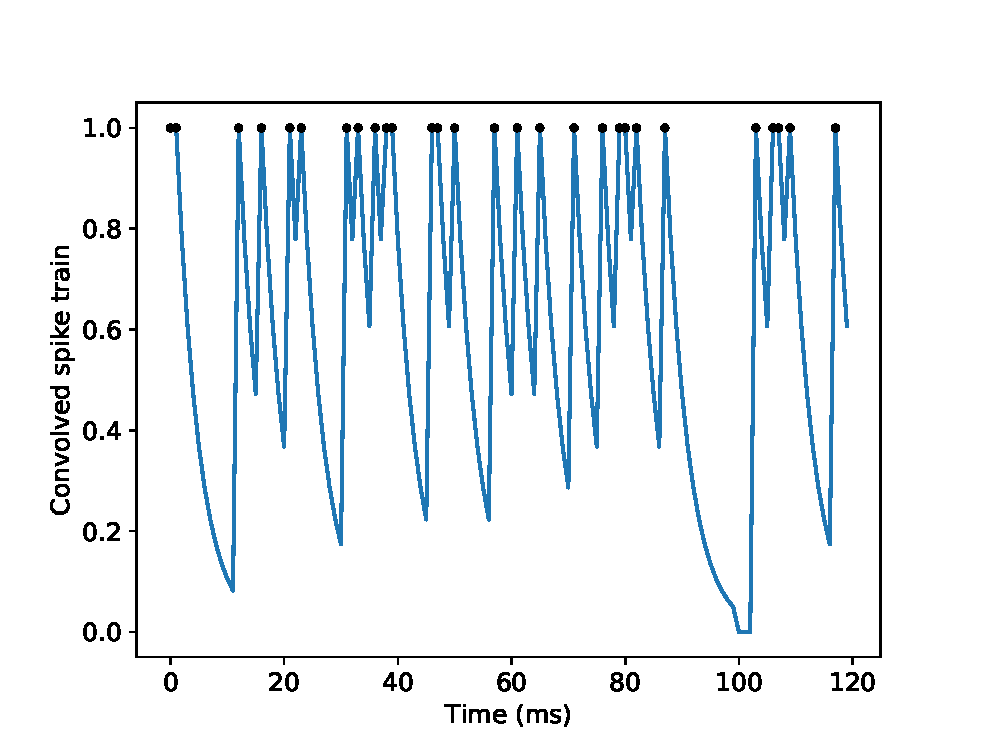
\includegraphics[width=0.9\columnwidth]{figures/samples/neur_vr_conv_sample.eps}
    \vskip -0.1in
    \caption{placeholder: van rossum convolution example}
    \label{fig:vrd_conv_sample}
    \vskip -0.2in
\end{figure}


% \subsection{KL-divergence}

% "different prob dists"

\subsection{Maximum Likelihood Estimation}

% Negative log-likelihood (Bernoulli, and Poisson PDF assumptions) for probability-based models.
By assuming either a Bernoulli or Poisson distribution for the observations, or spike trains, we can maximise the likelihood of producing that same data by using numerical methods.
As usual, it is easier to work with a sum of products, rather than exponents, when doing numerical differentiation over a probability distribution to find the maximum likelihood estimate (MLE).
Therefore we maximise the log-likelihood over the distribution, as it lets us work with a sum of products instead of a product of exponential functions, and is equivalent to maximising the likelihood itself.
In fact, we also instead minimise the negative log-likelihood, which remains equivalent to maximising the likelihood, as this lends itself directly to optimisation as a loss metric and error signal which may be used for gradient-calculation.

\begin{equation}
    \mathcal{L}(\theta | x) :\propto - \log \mathcal{L}(\theta | x) = - \log \prod_{n=1}^N pdf(\theta; X) = - \sum_{n=1}^N \log (pdf(\theta; X))
\end{equation}

Assuming a Bernoulli distribution,

\begin{equation}
    Bernoulli(\theta; x)
\end{equation}

Assuming a Poisson distribution,

\begin{equation}
    Poiss(\theta; x)
\end{equation}

These let us estimate the ML for $\theta$.




% -----------------------
% \subsection{Relaxing the constraint of differentiability}

% mostly if EAs??
% non GBO, but still ABC.

% permutations

% ...

% high-cost, not necessarily better due to stochasticity. 

% unknown input.

% may be studied further, but would require a large amount of computational resources, and it is currently unclear whether such endeavours would be fruitful. % ..?

% ---------------------
% \textbf{Something you can learn about network, but also should be specific to a spiking net
% Want to find something only in SNN, but which is also identifiable
% Don’t need to find exact same sync act., not same identities of neurons which participate, just general properties, in spite of unknown input activity}

% Advantages of SNNs compared to rate based/mean field
% Quantity
% Model statistics exhibited regardless of configuration
% Different inputs and generative model output variability

% “Vector strength is the Fourier component of the spike sequence at the stimulus frequency normalized by the total number of spikes”

% “It has been proposed that membrane time con- stant, spiking threshold, and the number of inputs per period are key parameters that determine the performance of a coincidence detector (Kempter et al. 1998)”
% On temporal info coded by phase-locked spikes processed in higher-order centers in the brain

% Precise firing sequence
% “Inappropriate surrogate” - high-order gamma dist great number of chance patterns due to generating quasiperiodic spike trains. Poissonian more unrelated periodic spike trains
% “Nonprecise time patterns” - interested in spike patterns (not one less precise peak in 3d corr M)

% (Analysis and interpretation of interval and count variability in (single neuron) neural spike trains
% Coefficient of variation (CV), trial-by trial count variability with the Fano factor (FF), estimation bias, …
% Variability on tens to hundreds of ms
% CV = SD(X)/E(X))

% Can we detect statistics relating to state in data using more sophisticated rate measures when compared to straightforward mean binned rates per state? Could this be used further?

% System. Spike train assumed to be distributed according to some distribution. Can invert and calculate probability and minimise. Fluctuation can for instance be regarded as due to “irregularity in time from a constant rate or regularly from a fluctuating rate”.
% Metric measuring ISI variability rescaled locally in time can suggest which is more plausible.
% When looking at more complex system this is less trivial..? MIght be used on higher-level such as neuron classes?

% Need to go beyond renewal processes to capture different neuronal modes of behaviour, and spike train adaptation - serial correlations in ISIs is one such step
% Hidden Markov processes, drawn from distribution relative to state
% “Memory” in nesting the probability such that it depends on N preceding ISIs

% Grün and Rotter, methods
% Characteristics that are stable in spite of different inputs

% Null hypothesis: Independence (spike trains)
% stochastic spike train models, posits probabilistic model for timing of spikes, based on the spike history. Simplest such; Poisson process.
% p(spike\_[t, t+dt]) ~~ Rdt, where R is the rate (for sufficiently small dt)
% Point processes for several spike trains (networks and not just neurons); papers (ignored here)
% ---------------------


% =======================================================
\chapter{Work: The frontier of SNN inference}

In order to study how to infer spiking neural network models (SNNs) one needs several ingredients: (1) a definition of the entire system, (2) an implementation of it, (3) an algorithm for model inference where (1) and (2) are compatible with the algorithm, and (4) a way to measure and assess model performance, ideally compared with existing methodologies and models.

Research on SNNs using gradient-based optimisation is fairly limited, and includes approximate Bayesian computation for smaller models, conversion learning in which more traditional ANNs are transformed to simpler SNNs after training, or surrogate gradient descent, in which a surrogate signal over the model spikes, usually as a function over the membrane potential, is used in order to obtain a differentiable output that may be used to optimise the model's parameters over a given loss metric by backpropagating the error signal.
% Currently, the state-of-the-art methods are only partly successful in training a subset of SNN model parameters for smaller models.
With the goal of accelerating SNN inference research, I looked at the most prominent state-of-the-art methodologies for SNN inference, which may be divided into (1) gradient based optimisation (GBO), and (2) approximate Bayesian computation (ABC) \cite{Lueckmann2018, Rene2020, Cranmer2020a, Lueckmann2021}.
GBO enables leveraging recent ML advances from deep learning, and albeit biologically implausible as a learning rule, allows for in-place model inference training and inference. The computational cost of doing gradient based computation is also exponentially less than that of doing ABC, as this involves doing a Monte-Carlo sampling step \cite{Rene2020}.

Previously, Bayesian inference was intractable for SNN models due to their high-dimensional parameter-space, but recent advances in sequential neural estimation techniques, where a DNN is trained to estimate a prior using a relevant statistic, has allowed for much more efficient sampling using this amortised approach; sampling from the DNN to perform posterior parameter estimation.
Note however that this procedure still has a high cost, which does not scale well with an increase in the network size.
% references, brief summary and discussion of main references
Using a Bayesian approach, we may however estimate the posterior over the model parameters, given our approximation of the prior. This also yields a type of uncertainty estimate around the posteriors. Note however that the posterior will be skewed by the prior approximation, in our case given by sequential neural ratio estimation (SNRE) \cite{Lueckmann2021}.
 
Using a surrogate gradient approach, we may fit the parameters of the system by error minimisation using any differentiable loss function. Due to the constraint put forth by working with biological spike train data, which is a very widespread format in which there is a vast amount of data available, we cannot however make many assumptions about the input, unless the recording somehow also contains information about this signal. 
Therefore, we have to include the input in the model, by making assumptions about the network input, as well as to consider how it may greatly affect network behaviour during learning. As a rule of thumb, we want to have a signal which allows for the network to perform the task at hand, or to replicate the observed data, whilst being as biologically reasonable as possible.
We want to have input that puts the system in a realistic mode of behaviour, and allows us to optimise its parameters such that an informative signal is transformed in a meaningful way.
% As it is limited what we may assume about the input, loss metrics that put a high emphasis on the precise timing of spiking may in fact obscure the gradient signal by incorporating too much of the noise stemming from this signal.
% We therefore focus on metrics that are more rate-based, looking at intervals of spikes in order to include the temporal signatures to some extent.
% Using a timing-oriented metric over larger time bins may even result in divergence, due to variability between the hidden target data input, and the inferred model input. 




% \section{My contribution: Implementing, differentiating and optimising different SNN models using different loss metrics}
\section{GBO compatible SNN framework in Pytorch}

Goals and questions or hypotheses
Novel method developed for advancing SNN inference by using gradient descent
Binary in nature, by implementing surrogate subthreshold spike signals, we may facilitate optimisation, improving optimisation performance for gradient descent.
We will retrieve a local minimum which is not approaching ground-truth in terms of model parameters, however, the model will capture the spike statistics to a greater extent than other models. As such, it may be used to evaluate the functional characteristics of the modeled nuclei.
The input is unknown.
SBI approach for SNN inference; limitations. Test potential.
Better for true parameter estimation. However,  posteriors are probability densities, and do not have direct access to full model configurations as such, and may suffer from not capturing full specific model configurations that capture as many higher-order spike statistics.
GLMs as a baseline to have comparable results for NMF analysis
% Input transformation (?, avg. relative spiking per population ?)
% net(x\_forward)
% Output transformation (avg. v per pop.)
% Can transform spike-train to average population membrane potential
% Synapses with dg/dt ?
% self.g = torch.ones\_like(self.v)  for one conductance per neuron (for n synapses)

% \subsection{Contribution: PyTorch}

% ... tricks, sequentiality etc
Current implementations of SNNs are commonly done in Brian 2 or Matlab. Upon commecing work on SNNs using LIF neurons, the only recent work we found that supported optimisation in a supervised or semi-supervised manner was in Theano, a legacy Python library.
With recent advances in ML not only through increased computational resources and novel optimisation techniques, but also in programming libraries which may be run using the GPU, and in either case contains highly optimised library code implemented in a lower-level programming language (for Python typically C or Cuda), I wanted to make use of this aspect too, and after too many hours of fighting with at best poorly documented Theano-library code, I decided to set out to implement SNNs in Pytorch.
This quickly led to the implementation of a modular pipeline and framework of SNN inference using GBO in Pytorch.
It also required maintaining a neuronal state throughout simulation, for which I simply implemented sequential input forward-propagation thoughout the model, which would also mutate its state.
With this simple trick, intervals of input mutate the state with each input corresponding to some desired time-step constant, in my code set to $1 ms$ for simplicity. % TODO: SI unit
However, it does result in that intervals of simulation need to be performed for each backward pass, i.e. updating the model parameters given error gradients.

I implemented a general SNN optimisation framework on top of Pytorch \cite{Paszke2017} and utilised Pytorch's autograd-feature for backpropagation of error gradients.
Key to enabling backpropagation is defining spiking using a differentiable function, such as the sigmoid function, i.e.

\begin{equation}
    s_t(v) = \frac{1}{1+e^{-(v_t-(\theta_v + \theta_s)}}
\end{equation}

where $s_t$ denotes whether a neuron spikes at time $t$ with a membrane potential $v_t$. Or by considering the spiking to be a readout of a continuous parameter/variable such as the post-synaptic current from each neuron, as is done in the case of the continuous sub-threshold synaptic model in \cite{Huh2017}.

% ref. Adam
% synthetic data generation with pseudo-random Poisson input, data driven experiments in vivo data set.
To perform optimisation, an initial model parametrisation is drawn uniformly from parameter intervals that are constrained to meaningful parameter values, and then perturbed with input drawn from some input generator function. Note that the parameters of this function may also be fitted.
The model output is then compared with the output of a target data set, and the specified loss metric and distance is calculated between the produced model output and target spike train.

\subsection{The framework}

% Modular Python-based framework written in Pytorch that allows for automatic differentiation of the computational graphs defined with Pytorch-code.
I implemented a framework in Python/Pytorch, performing differentiation \& optimisation using the autograd-feature of Pytorch.
Further, Pytorch allows for compactly defining the models by using the library code, which again is compiled into a computational graph, which in turn is able to be compiled into and run using the pre-compiled C++ or Cuda library-code.
Note that as such, this does not only allow for automatic differentiation using the computational graph constructed by defining nodes, edges, and leafs in the graph, but model simulation itself becomes fast when only running library-code, and not escaping to the Python interpreter.
While a comparison of run-time speed is out of scope in this thesis, it is often possible to reach a level close to that of C/C++, or Cuda - but with a main bottleneck in this case being imposed by the temporal limitation of SNNs; namely that simulation must be done whilst maintaining the model state in time throughout each simulation interval.

For the framework itself, the code may be found openly available at \href{https://github.com/williampeer/snn_inference}{github}, I structured this into parts roughly divided into packages for models, analysis, utilities, experiments, and tests, with test coverage of most of the code.

One of the main entry points allows for selecting an experiment type, model type, loss metric, and optimiser, with plugging in an external data set being optional - if not a random target model of the same class as the set model type is used to generate synthetic data.


\subsection{Batching and SNNs}

Despite the need to do simulation in a sequential manner as described above, I implemented iteration over batches of activity, effectively allowing for a type of batch normalisation, and increasing the parallelisability of the algorithm with the number of batches run in parallel, allowing for better use of the computational resources at hand.


\section{Experiments}

Each experiment consists of fitting the model class at hand to two data sets; (1) a general data set synthetically generated by a hand-engineered GLIF model, which produces a rich array of behaviours and spike correlations, and (2) a target model belonging to the same model class, which has been determined to lie in a non-chaotic parameter regime.
This allows for comparing inference performance to both the same data set across model classes, as well as to measure the average parameter distance when fitting to the same model class for which the ground truth values are avilable.

% \subsection{Optimisation}

For each experiment, the model is pseudo-randomly initialised by first setting a random seed (such that results may be reproduced) and then drawing initial parameter values uniformly from pre-defined parameter intervals, which are set such that the model is in a non-silent mode, with the parameters being set to biologically plausible values.

Then, each model is fitted until either the average gradient has decreased to a fraction ($\approx 1 \%$) of the initial average gradient, or for a set number of training iterations, $N_{exp}=200$.
Each training iteration consists of model simulation for an interval of $t=1200 \si{ms}$, and then updating the parameter values according to the gradients.

Since some model parameters are more sensitive than others, I defined linear constraints for each parameter, which Pytorch allows for incorporating into the computational graph in a simple manner by defining a hook for each backward pass over the parameters, i.e. for each gradient update, effectively clamping the gradients such that the parameters do not wander outside of realistic intervals. These intervals are naturally far wider than the initialisation intervals, but by considering what intervals are realistic, this is a simple and natural way to exclude unrealistic modes of model behaviour whilst constraining optimisation simultaneously.

% SBI is also different from what René et al. did in their paper. So these are two methods to compare with their findings. 


\subsection{Results}

Prior to the main experimental setup above, I simulated each model class for realistic intervals of parameters, whilst fixing the other parameters to values that I had empirically or analytically determined to be able to produce meaningful output, and plotted the loss and rate when compared to the target model of the same model class, essentially performing a grid search over parameters allowing to plot the marginals of the parameter landscape formed by the loss metric and target model signal.
The results which are included below illuminate how optimisation traverses the gradients formed by the parameter landscape, and gives an idea about the extent to which the procedure is applicable to the model class.

% GLIF
\begin{figure}
    \centering
    \vskip -0.1in
    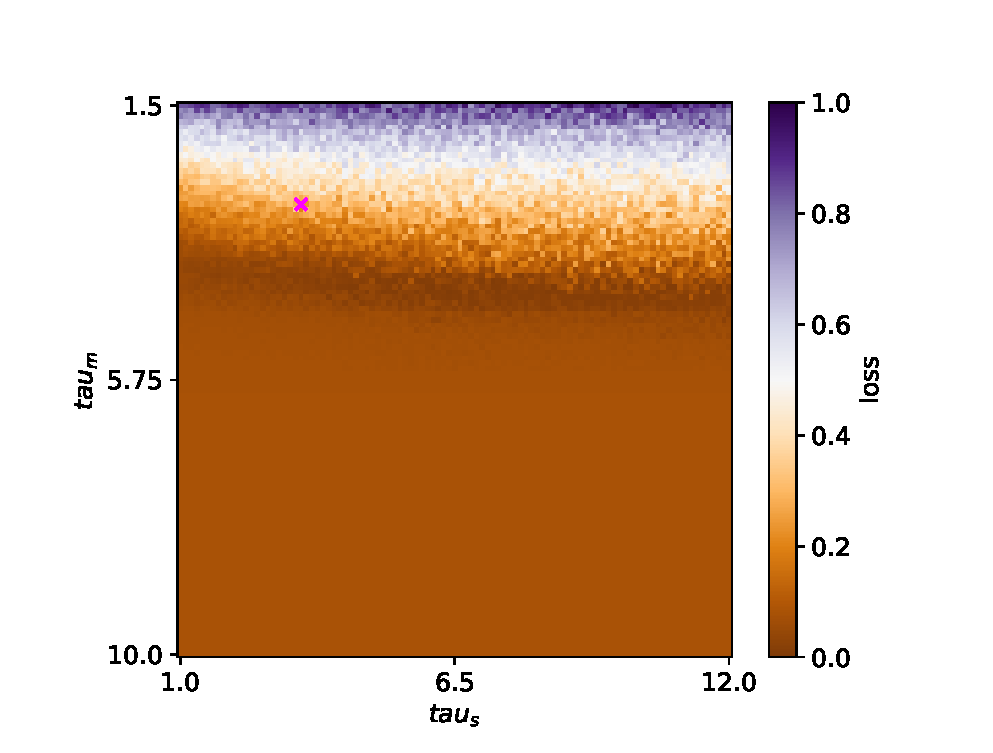
\includegraphics[width=0.9\columnwidth]{figures/param_landscape_heatmaps/GLIF/test_export_2d_heatmap_N_4_loss_tau_s_tau_m.eps}
    \vskip -0.1in
    \caption{p landscape GLIF tau s tau m}
    \vskip -0.2in
\end{figure}

\begin{figure}
    \centering
    \vskip -0.1in
    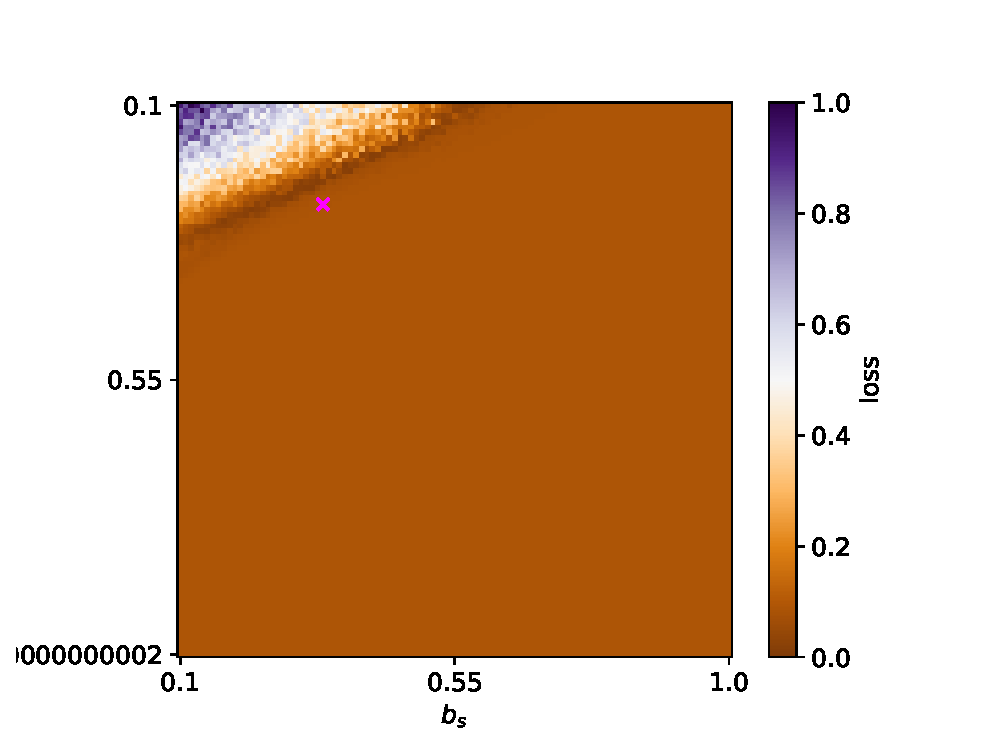
\includegraphics[width=0.9\columnwidth]{figures/param_landscape_heatmaps/GLIF/test_export_2d_heatmap_N_4_loss_b_s_a_v.eps}
    \vskip -0.1in
    \caption{p landscape GLIF tau s tau m}
    \vskip -0.2in
\end{figure}

% LIF
\begin{figure}
    \centering
    \vskip -0.1in
    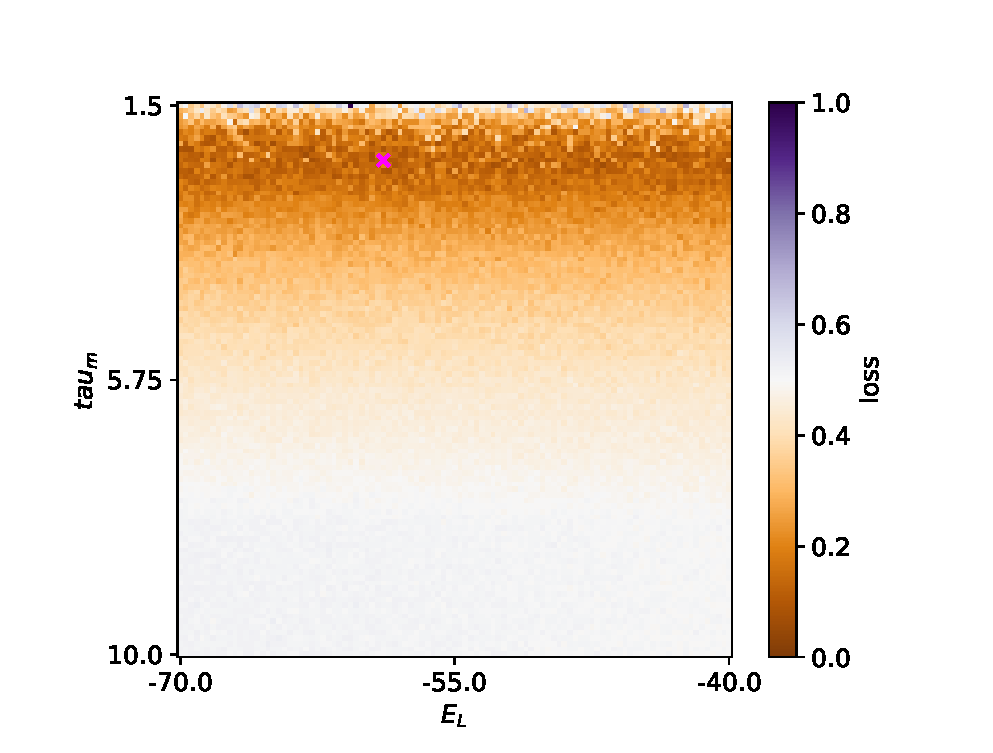
\includegraphics[width=0.9\columnwidth]{figures/param_landscape_heatmaps/LIF/test_export_2d_heatmap_N_4_loss_E_L_tau_m.eps}
    \vskip -0.1in
    \caption{p landscape GLIF tau s tau m}
    \vskip -0.2in
\end{figure}

\begin{figure}
    \centering
    \vskip -0.1in
    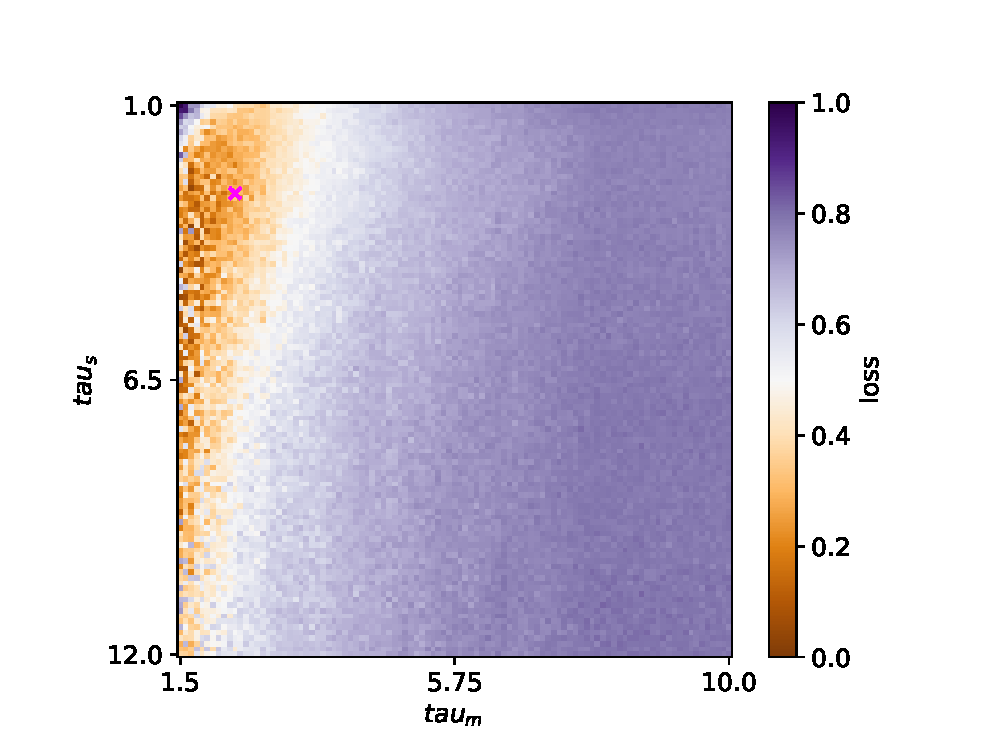
\includegraphics[width=0.9\columnwidth]{figures/param_landscape_heatmaps/LIF/test_export_2d_heatmap_N_4_loss_tau_m_tau_s.eps}
    \vskip -0.1in
    \caption{p landscape GLIF tau s tau m}
    \vskip -0.2in
\end{figure}

% mesoGIF
\begin{figure}
    \centering
    \vskip -0.1in
    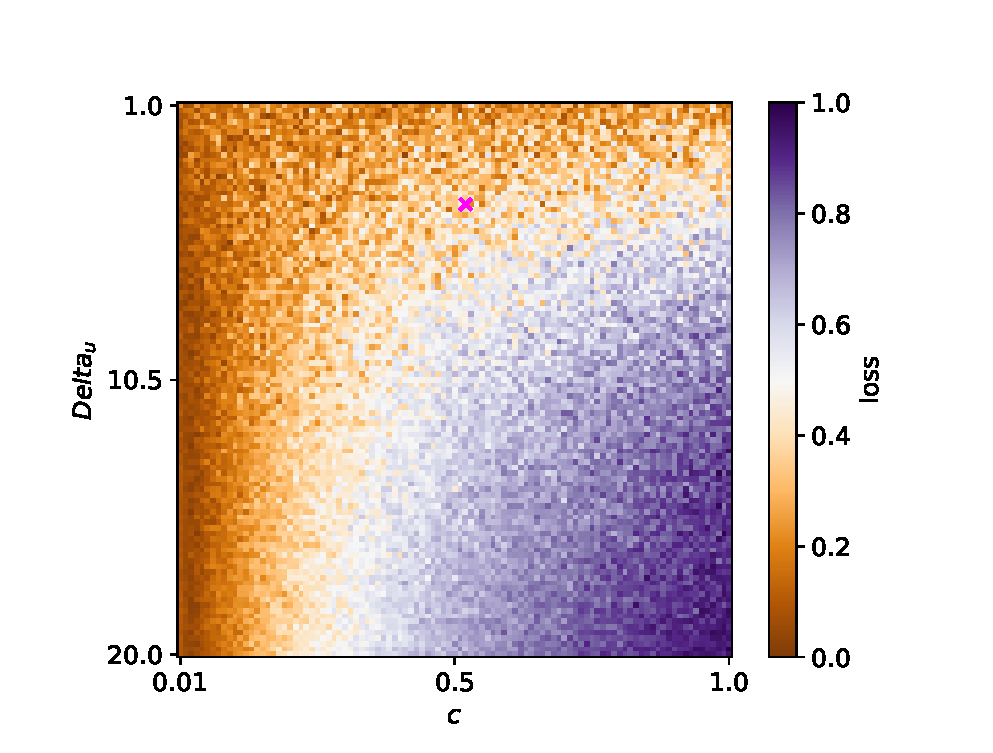
\includegraphics[width=0.9\columnwidth]{figures/param_landscape_heatmaps/microGIF/test_export_2d_heatmap_N_4_loss_c_Delta_u.eps}
    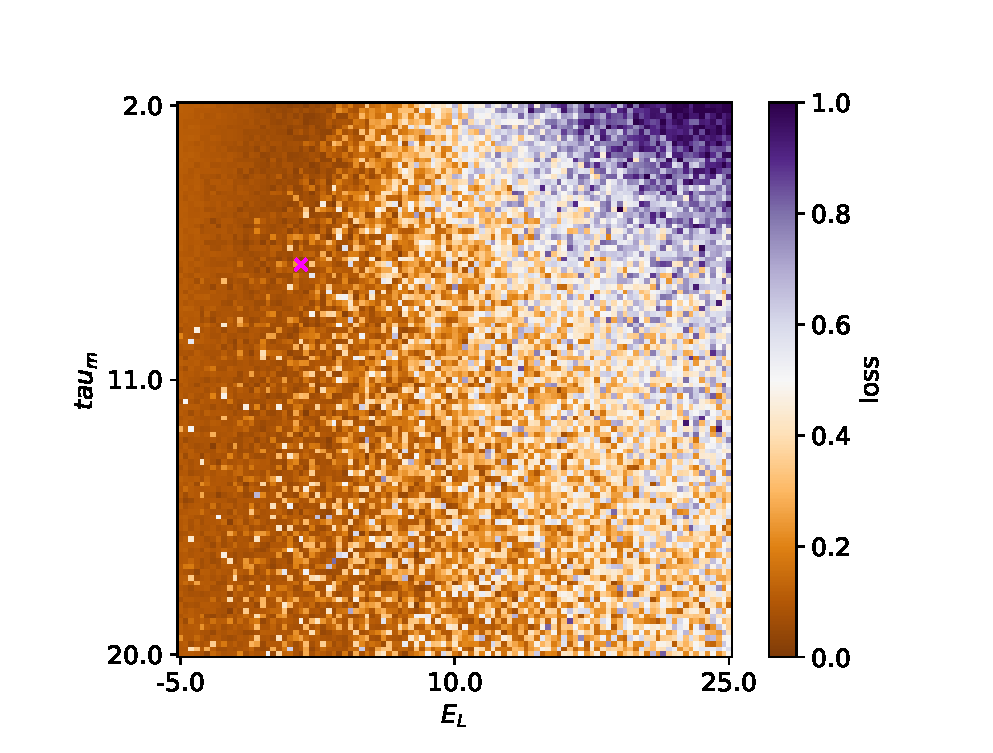
\includegraphics[width=0.9\columnwidth]{figures/param_landscape_heatmaps/microGIF/test_export_2d_heatmap_N_4_loss_E_L_tau_m.eps}
    \vskip -0.1in
    \caption{p landscape GLIF tau s tau m}
    \vskip -0.2in
\end{figure}

\begin{figure}
    \centering
    \vskip -0.1in
    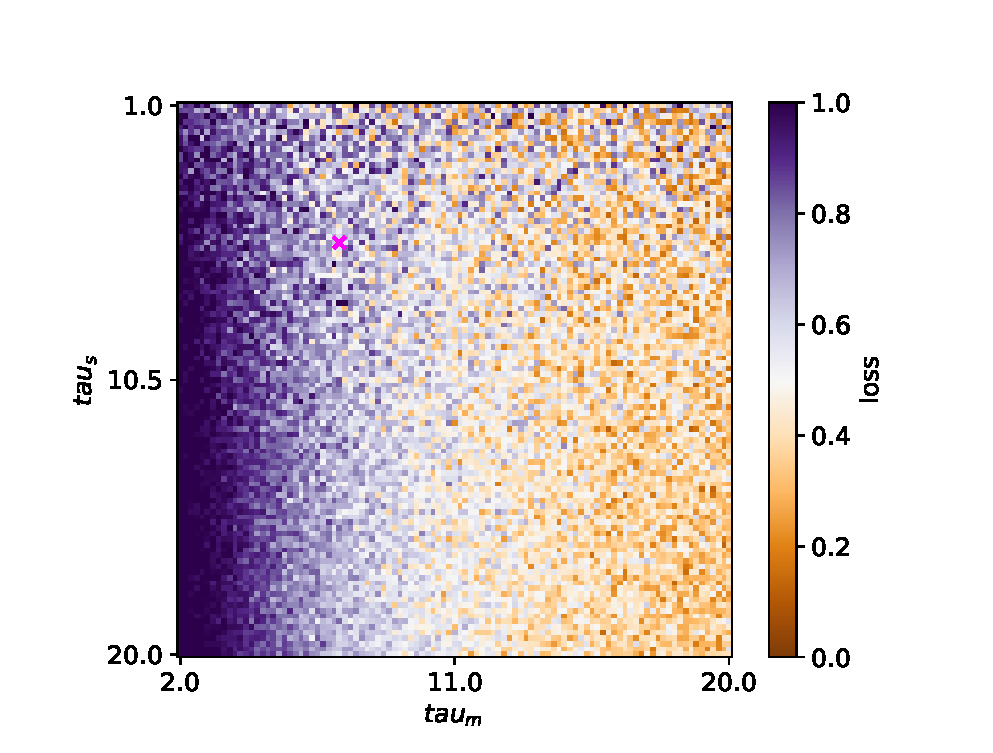
\includegraphics[width=0.9\columnwidth]{figures/param_landscape_heatmaps/microGIF/test_export_2d_heatmap_N_4_loss_tau_m_tau_s.eps}
    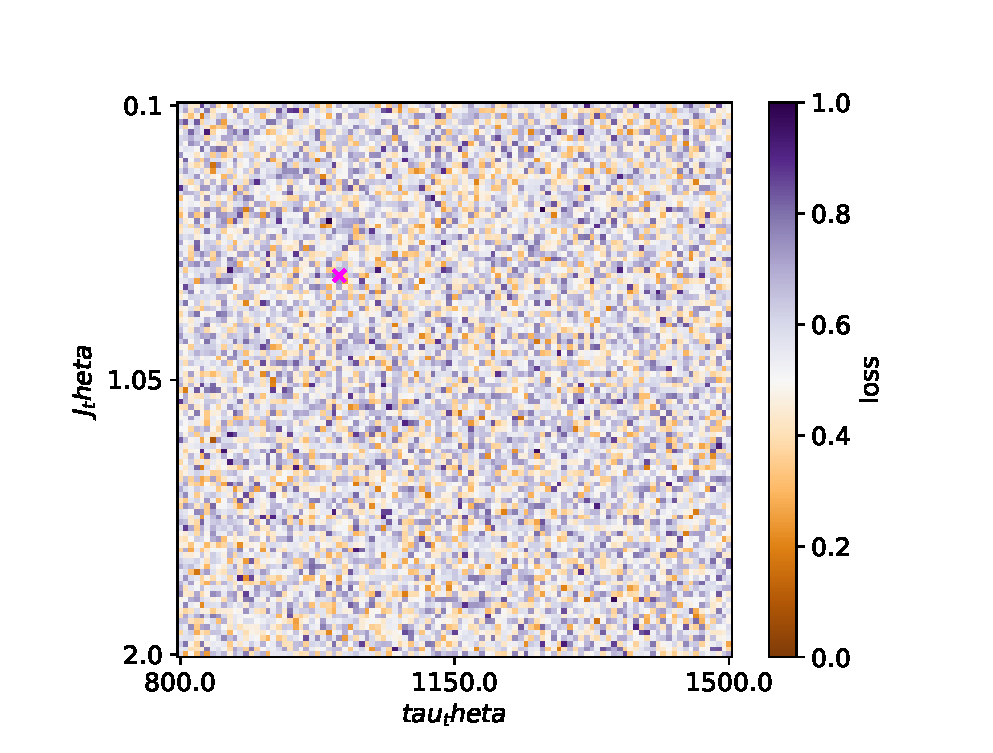
\includegraphics[width=0.9\columnwidth]{figures/param_landscape_heatmaps/microGIF/test_export_2d_heatmap_N_4_loss_tau_theta_J_theta.eps}
    \vskip -0.1in
    \caption{p landscape GLIF tau s tau m}
    \vskip -0.2in
\end{figure}
\begin{figure}
    \centering
    \vskip -0.1in
    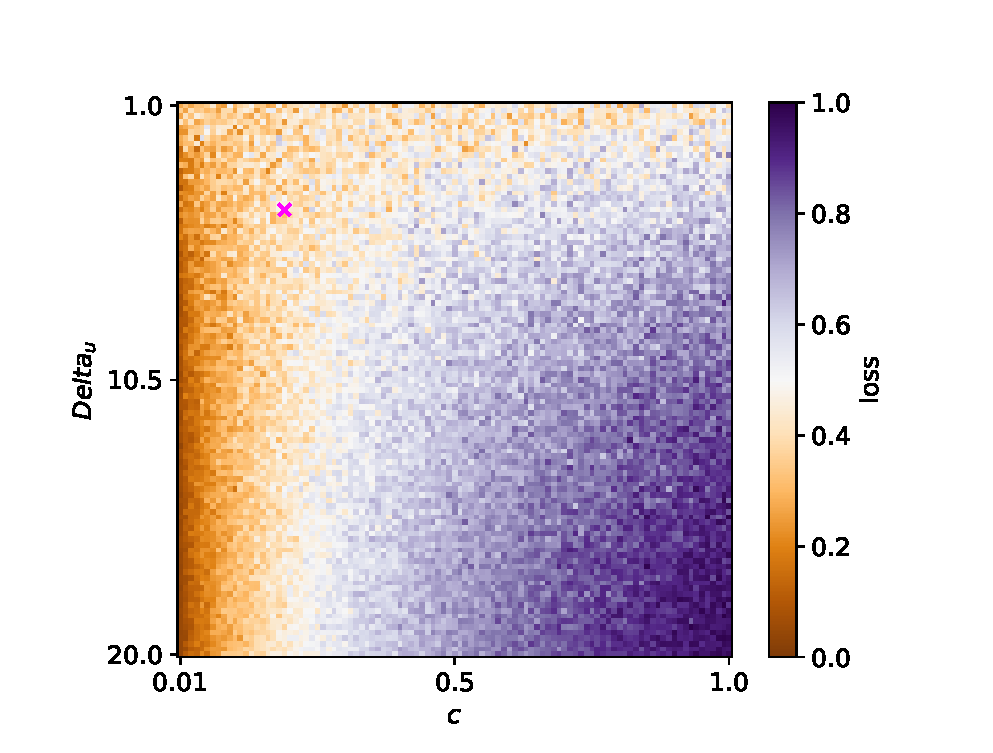
\includegraphics[width=0.9\columnwidth]{figures/param_landscape_heatmaps/microGIF/test_export_2d_heatmap_N_21_loss_c_Delta_u.eps}
    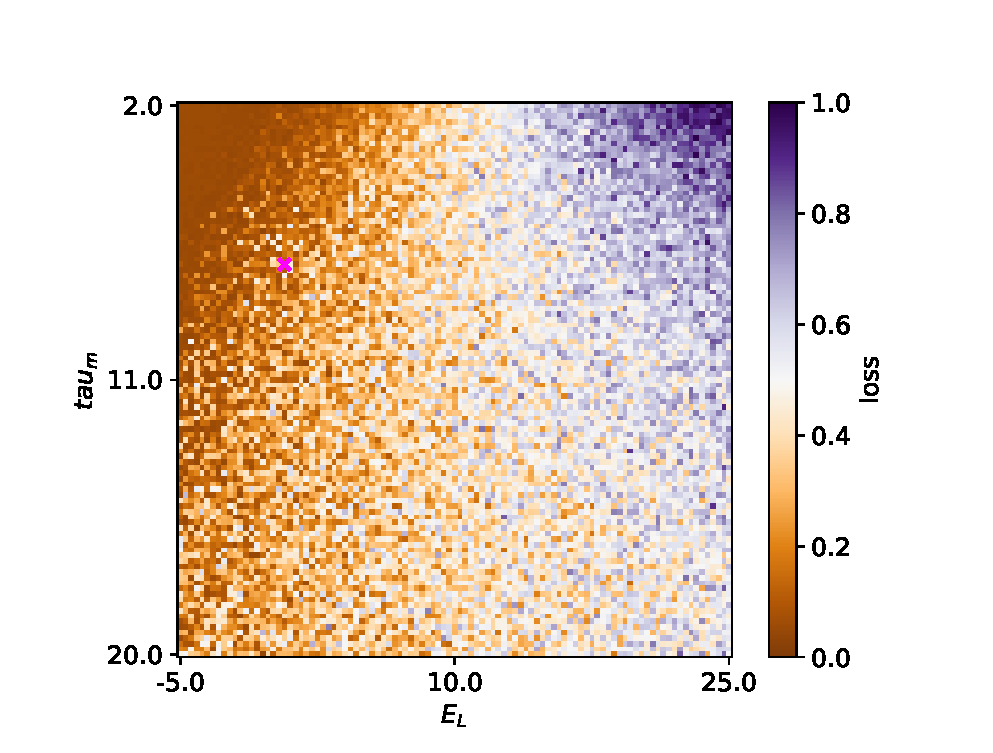
\includegraphics[width=0.9\columnwidth]{figures/param_landscape_heatmaps/microGIF/test_export_2d_heatmap_N_21_loss_E_L_tau_m.eps}
    \vskip -0.1in
    \caption{p landscape GLIF tau s tau m}
    \vskip -0.2in
\end{figure}
\begin{figure}
    \centering
    \vskip -0.1in
    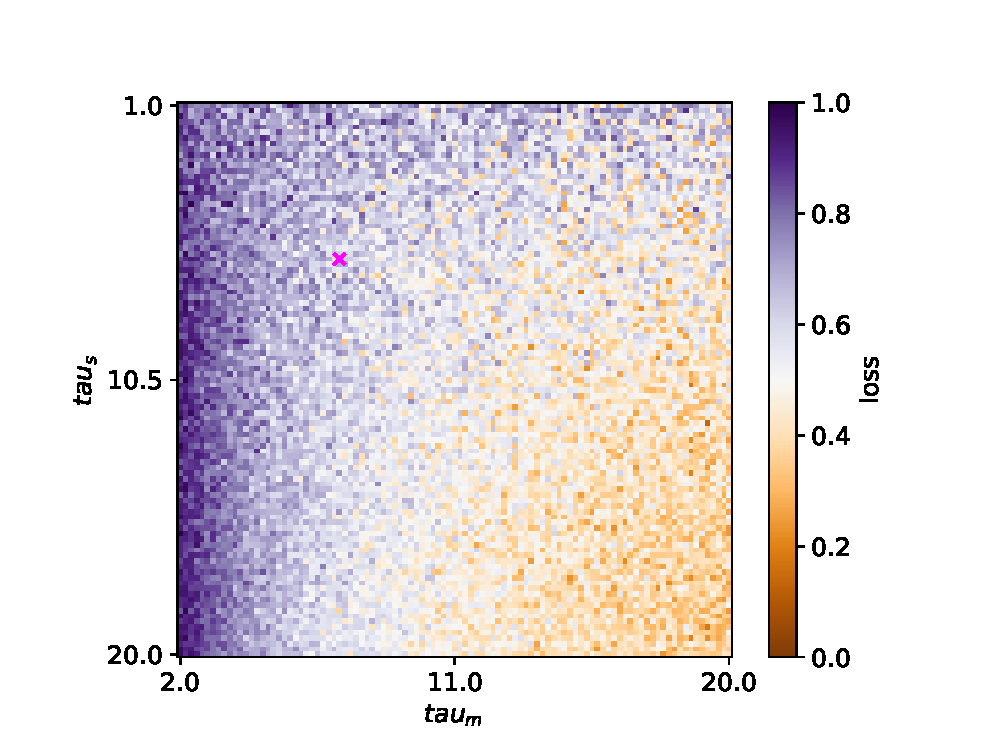
\includegraphics[width=0.9\columnwidth]{figures/param_landscape_heatmaps/microGIF/test_export_2d_heatmap_N_21_loss_tau_m_tau_s.eps}
    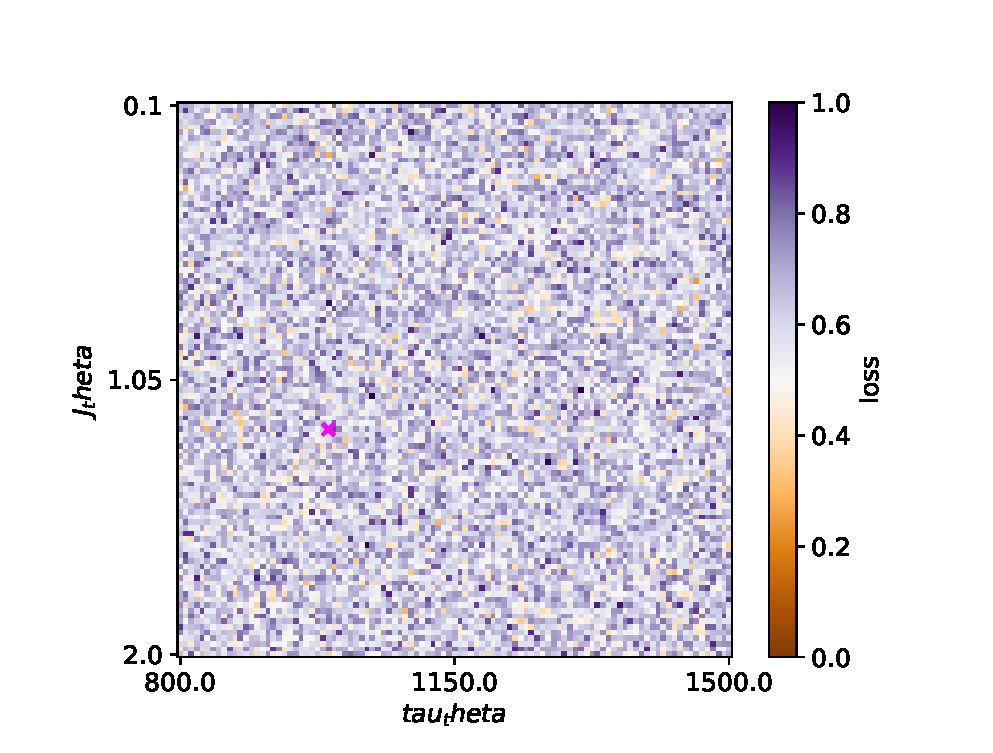
\includegraphics[width=0.9\columnwidth]{figures/param_landscape_heatmaps/microGIF/test_export_2d_heatmap_N_21_loss_tau_theta_J_theta.eps}
    \vskip -0.1in
    \caption{p landscape GLIF tau s tau m}
    \vskip -0.2in
\end{figure}

Description parameter landscape plots. Spaces for which error gradient given by frd metric is amgbiguous, i.e. wanders arbitrarily, and is thus not satisfactory in terms of retrieving the ground-truth. 
However, for the vrd, these are even more obscure and noisy... (plot generation if time)

For Izhikevich: <inser description>
Therefore not included in GBO experiments.

% Experiments:
% SameModelClassTarget
\subsection{Known ground-truth synthetic data}
Fitting to synthetic data generated by the same model class, such that we may compare the retrieved parameters with the ground truth.
Data was generated by hand-engineered models of the same class as the model being fitted (i.e. LIF, GLIF, or microGIF).

\begin{figure}
	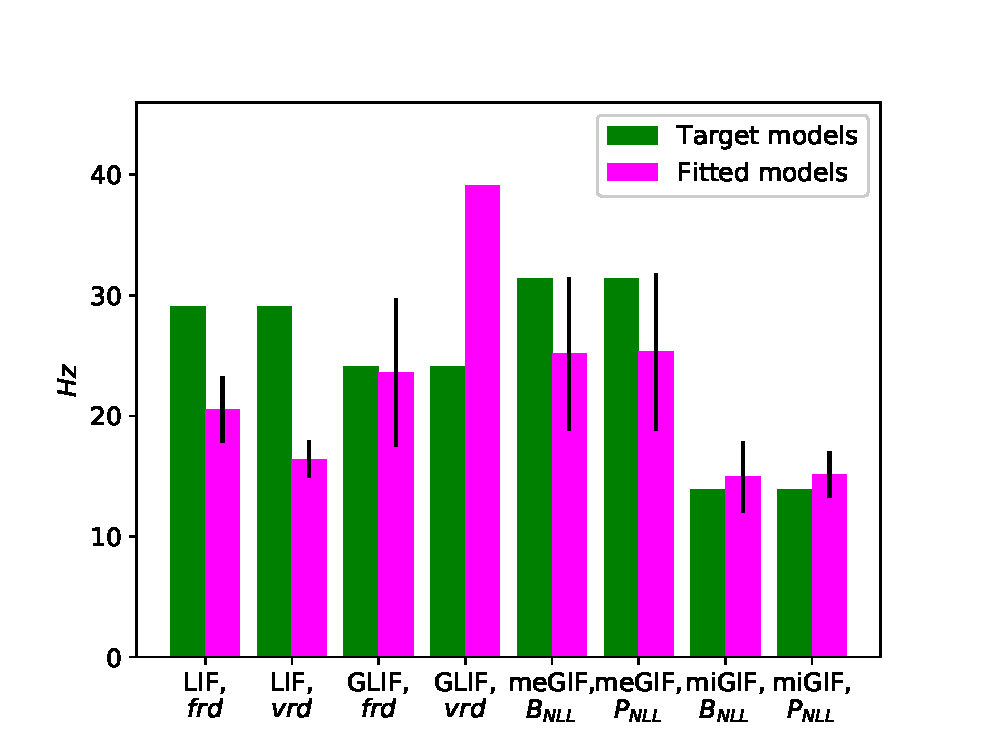
\includegraphics{figures/export_rates_saved_all.eps}
\end{figure}

\begin{figure}
	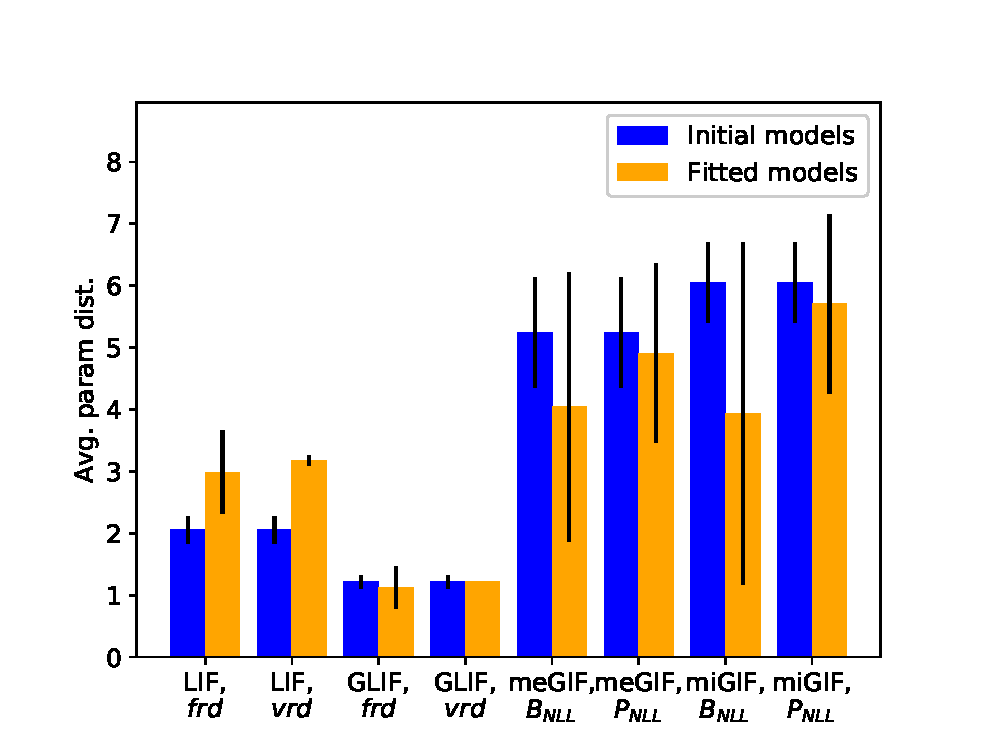
\includegraphics{figures/export_p_dists_saved_all.eps}
\end{figure}

%sample microGIF poisson & bernoulli
% export_microGIF_plot_loss_euid_12-09_16-36-58-996.eps
% export_param_inference_X_microGIF_1_E_L_.eps
% export_spike_trains_euid_12-09_16-36-58-996.eps


\subsection{Shared synthetic data set across model types}
Fitting to the same synthetic data set, such that we may compare performance across model types for the same data set. 
This data was generated by a hand-engineered ...

\begin{figure}
	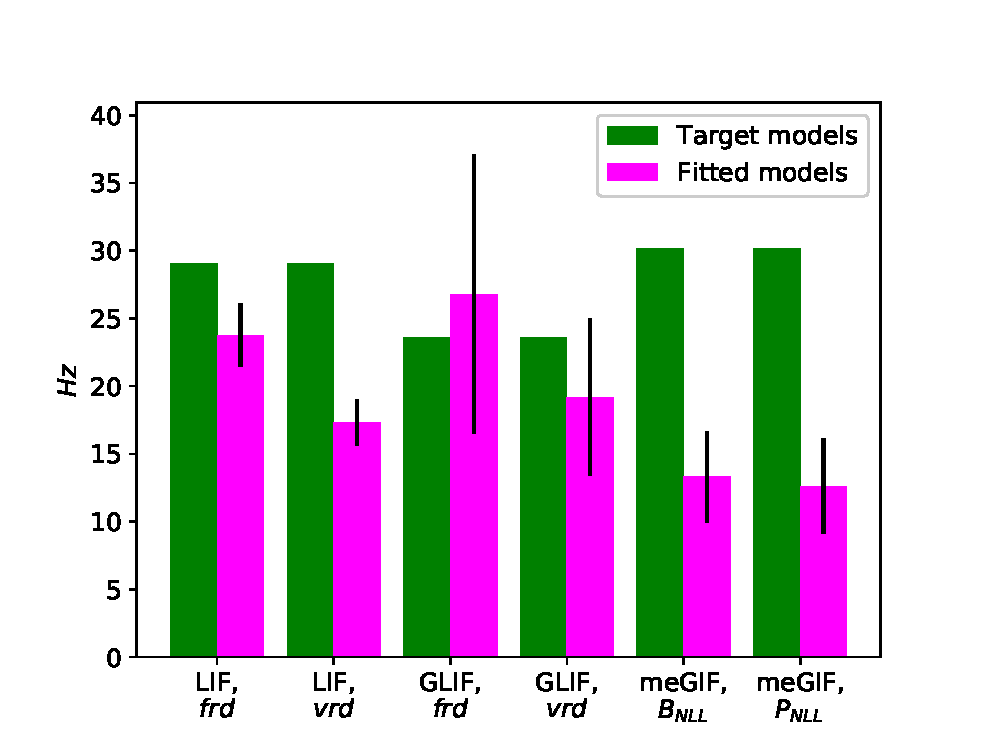
\includegraphics{figures/export_rates_only_GT_all.eps}
\end{figure}

% \begin{figure}
% 	\includegraphics{figures/}
% \end{figure}

\section{Simulation-based inference}

Using the best performing loss-metric as found in the GBO experiments, and also revealed by the parameter landscape plots, i.e. the firing rate loss metric, we performed SBI by using the Python-framework of the Macke-lab \href{https://github.com/mackelab/sbi}{SBI}.

% sbi_p_avgs_pairplot_SNPE_GLIF_12-15_14-22-38-919.eps
% sbi_p_avgs_pairplot_SNPE_LIF_12-15_04-56-19-338.eps
% sbi_p_avgs_pairplot_SNPE_microGIF_12-14_16-14-12-736.eps

% General description across p-dists, and mostly rates (implicitly loss).

\section{NMF analysis}

% \begin{figure}
% 	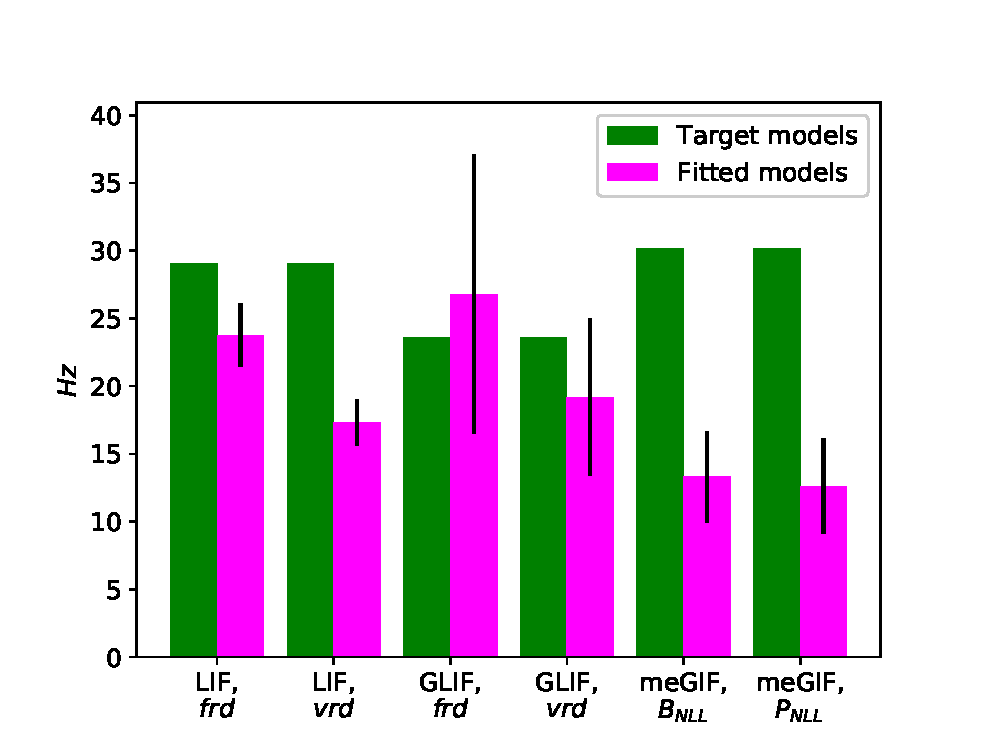
\includegraphics{figures/export_rates_only_GT_all.eps}
% \end{figure}

% bugged_mesoGIF_4.eps
% bugged_microGIF_4.eps
% bugged_microGIF_21.eps
% export_GLM_filters_pred_bin_size_0_1_cell_2_target_GT_model_GLIF_N_4.eps
% export_GLM_filters_pred_bin_size_0_1_cell_2_target_GT_model_LIF_N_4.eps
% export_GLM_filters_pred_bin_size_0_1_cell_2_target_GT_model_mesoGIF_N_4.eps
% export_GLM_filters_pred_bin_size_0_1_cell_2_target_GT_model_microGIF_N_21.eps
% geodesic_distances_Synthetic_GLIF.eps
% geodesic_distances_Synthetic_LIF.eps


% \subsection{Leaky integrate-and-fire (LIF)}

% Gradient-based methods prone to finding sub-optimal solutions, i.e. local minimas. This is an issue particularly for high-dimensional feature spaces. Thus, I am led to believe this will be an issue when trying to infer the model parameters of complex neural networks using spike trains.

% %--------------------
% LIF work log:
% More nuanced
% Very noisy gradients for unstable/chaotic generative model perturbation?
% Dynamic R\_I in conjunction with frd might result in better convergence, due to constraining search space.
% By using dynamic R\_I (linear constraint), this makes behaviour more stable, and so may allow for more calibration/optimisation of the other parameters.

% % vRD suddenly seems viable for more stable network behaviour. When model behaviour was more chaotic, frd was better. This makes sense, as gradient will not be well-defined for vRD when model is chaotic. Not necessarily for frd either, but this is more robust to noise.

% Some artefacts LIF (more linear, easier to have whole-network spiking with too little inhibition / simpler neuron dynamics)

% Initial conditions large effect on convergence

% vRD performance OK with tau=100.0
% frd better
% In conjunction: still sometimes silent neurons. Potentially due to local minima of vRD for silent neurons, and obscured parameter-landscape due to noise and the nature of the vRD-metric. Not necessarily orthogonal to frd either, and as such may interfere with its gradient

% Will have to look at vRD vs frd vs frd+vRD vs adaptive(frd+vRD) quantitatively for setups.

% There seem to be many regions for which there is no “information gain” when moving along gradients, such as for silent neurons. Some parameters might not have their effect obscured or less pronounced due to the change of other parameters in parallel, too. This is the reason other authors have performed sequential parameter optimisation.

% When constructing generative target models, we aimed for hand-engineering models entraining higher-order ensemble dynamics that were stable across different random seeds of model perturbation, such that we could test how well model inference would capture these statistics. To this end, we designed three populations of neurons, where each population had different neuron parameters, normally distributed around set means, with a standard deviation of 25 % around the population values for each neuron. 
% In order to not generate spurious data, such as if the generative model is driven primarily by its input perturbation, or where it behaves otherwise chaotically, we tested that the hand-engineered models’ higher order statistics indeed occurred across different random seeds.

% (To verify that the model would indeed be sensible for synthetic generation, we tested the stability of neuron rates across different random seeds. When a deviation lower than X was attained, we accepted the ensemble model as a generative model suitable for data generation in order to test our framework.)
% Note that this deviation test is only to determine that the model doesn’t behave chaotically, and does not fire spuriously, in which case optimisation would be like fitting to noise, which should not converge.



\section{"Cortical microcolumn"-inspired stochastic population integrate-and-fire models}
% \subsection{Contribution: microGIF work}
\label{microGIF}

Based on the work of \cite{Rene2020}, which is based on \cite{Schwalger2017}.
Spike probability, rather than membrane potential and spikes.
--> Minimise negative log-likelihood under a Bernoulli or Poisson assumption.


% TODO: check: "frontier" found using frd - vrd obscures gradient and diverges more.
BNLL \& PNLL "frontier"

% \subsection{GLIF neurons}
% Can be highly parameter-sensitive and result in completely different mode of neuronal behaviour


\subsection{Loss metrics}

% Tricky design, stochasticity, lots of considerations, as we shall see only frontier..
When it comes to designing suitable loss metrics, this is one of the main challenges for applying gradient based optimisation to SNNs, as it is what defines the gradients, and thus the parameter space that we traverse during optimisation.

% figures of parameter landscapes


% \subsubsection{van Rossum distance}
Hypothesis: Using the van rossum distance may guide search, allowing gradient-based methods to converge?

Using the van-rossum distance as a loss function for the spike trains, we get something more continuous, since the discrete spike train is convolved with a time-based kernel. 
This should make the gradients more informed via the loss function in larger search areas.

% figures of a convolved spike train, reference to LIF poster

% for probabilistic SNNs, as well as GLIF(?) SNNs:
Main finding: 
"\textit{wandering gradients}" for vRD.

One thing is quantifying distances in terms of spike metrics.
Another is designing a metric that is well-defined for gradient-descent.
While the van Rossum metric describes the distance between two spike trains both in terms of rates and timing, due to its sensitivity to exact timing the gradient signal might be obscured for non-matching neurons, and more well-defined where the rates better match.


\subsection{\textit{Best-effort GBO with input-specific parameter regime(?)}}


\section{Discussion}

\subsection{Stochasticity and SNNs}


\subsection{Model input perturbation and formulation}

Task: Model site from which spikes have been recorded and decoded. Issue: We don’t have the input to the site. Options: Auto-encode temporal evolution of spike train, or infer model to produce outputs when noise-driven. Question: Is this at all attainable?

Learning methods:
BP, BPTT, Surrogate gradient (what we’re doing), soft-threshold (very similar to what we’re doing, but not in-place), STDP (has similarities, but not what we’re doing - more suitable to local and temporal learning?)

One finding is that we can infer a LIF SNN capturing higher-order statistics with a noise-driven setup (during inference). Using more temporally oriented loss functions quickly becomes problematic due to the input-noise, however. Can we show this analytically or empirically somehow for more complex models?
Another scheme: Predict next input given previous - (learn patterns from the information we have) then predict when perturbing with noise. Would also allow for hand-engineering input with different qualities (inspired by vigilance/sleep state), and test whether functional ensembles resemble those observed during these states in vivo.

Given the learning algorithms that we have available, how detailed spiking models may we infer by using common data sets? More specifically, can we increase the level of detail and level of higher-order statistics captured in a model by also inferring internal neuron variables by using gradient-based optimization? Is this possible by only using a one-dimensional target signal, such as spike trains? Does more detailed neuron models than LIF models enable capturing a higher level of detail and statistics, through allowing a wider array of model behaviour? Can we fit these models in a noise-driven scheme, such that the approach may be used on real-world data? If not, what are our alternative approaches? Could we for instance fit to output data given previous output data, i.e. similar to auto-regression? If so, would this enable us to predict output under different brain states?
Model inference should be compared to common statistical models, including GLMs, Gaussian mixture models, and Poisson models.


Method assumes access to observed neural activities and external input.
René et al. (2019/20) paper:
“The method we present assumes that the model to be inferred can be expressed as a
set of stochastic equations and that we have access to time series for both the observed (and possibly aggregated) neural activities and external input”


\subsubsection{Sine modulated white noise input}

\begin{equation}
    \sum^M sin(W(t))
\end{equation}

\subsubsection{White noise input}

\begin{equation}
    W(t) \sim \mathcal{U}(t, m)
\end{equation}

\subsection{Multi-layer versus single-layer SNNs}

Multi-layer net crucial for non-linear function approximation! We have not had this. If we only wish to capture the spike statistics, then a multi-layer version training on the next spike given the previous could perform better than the current single-layer noise-input to spike output?
What we have tried is instantaneous reactivity given noise-input. Is this not largely spatially oriented? To include a more temporal orientation, we may need to redesign the setup.

Auto-encoding task of own readout would make sense. However, we only have the binary spike output, and not continuous membrane potential


\subsection{Negative results}

Optimisers, parameter landscapes, hyperparameters, (linear) parameter constraints, input-output data, model topology and recurrence.

Preliminary conclusion: The spatiotemporal nature of SNNs, with the main measured effect being a function over a highly composite variable that has a high temporal dependency and thus variability, makes optimisation largely unsuitable with the current common definitions of optimisation algorithmics, including the loss metrics mentioned in this thesis.
In addition to being highly sensitive to initial conditions and other factors potentially both skewing the times of spiking, as well as the very mode of behaviour and spiking, input-output transformations, and the spatiotemporal signature of spike trains, need to be handled in a way that is more robust to these perturbations. 
Currently, there seems to be no defined loss metric that may capture the distance and resulting parameter landscape when going from one mode of behaviour to another in network nodes in a way that is exploitable by means of gradient based optimisation.

\subsection{Future work}

So how, then, can we ameliorate, or solve automatic model inference for accelerating (computational) neuroscience research?

Below is a list of points summarising observations that I made during my research that may be useful to have in mind for future research in the area.

\begin{itemize}
    \item Measure input activity, or model this in a meaningful way.
    \item Work with well-defined input-output transformations.
    \item Work with multi-layer networks - although these are then non-linear and less straightforward, they may constrain state space (hypothesis?)
    \item Constrain parameter intervals as much as possible using sensible intervals (such as when looking at probable cell type mixtures using the Allen Brain DB)
    \item Perform early population level or average comparisons to determine whether setup is indeed suitable for GBO model inference
    \item Preliminary model results can be verified using approximate Bayesian approaches
    \item Consider using non-leaky models to greatly constrain model behaviour and thus facilitate GBO
    \item Using a subthreshold synapse model enables subthreshold continuously differentiable signals over the synaptic currents, allowing for optimisation for instance in "silent" models with subthreshold synaptic currents, and potentially improving optimisation
    \item There needs to be a transformation of the IO which brings the model into a stable regime suitable for GBO
        Linear transformations are good alternatives for this, and can save one for a lot of hand-calibration in order to attain a regime in which GBO is well-defined/does not diverge
\end{itemize}



% =======================================================
\chapter{Gradient-descent based LIF SNN inference}
\section{Poster: \textit{Spiking Network Inference Using Gradient Based Optimisation}}
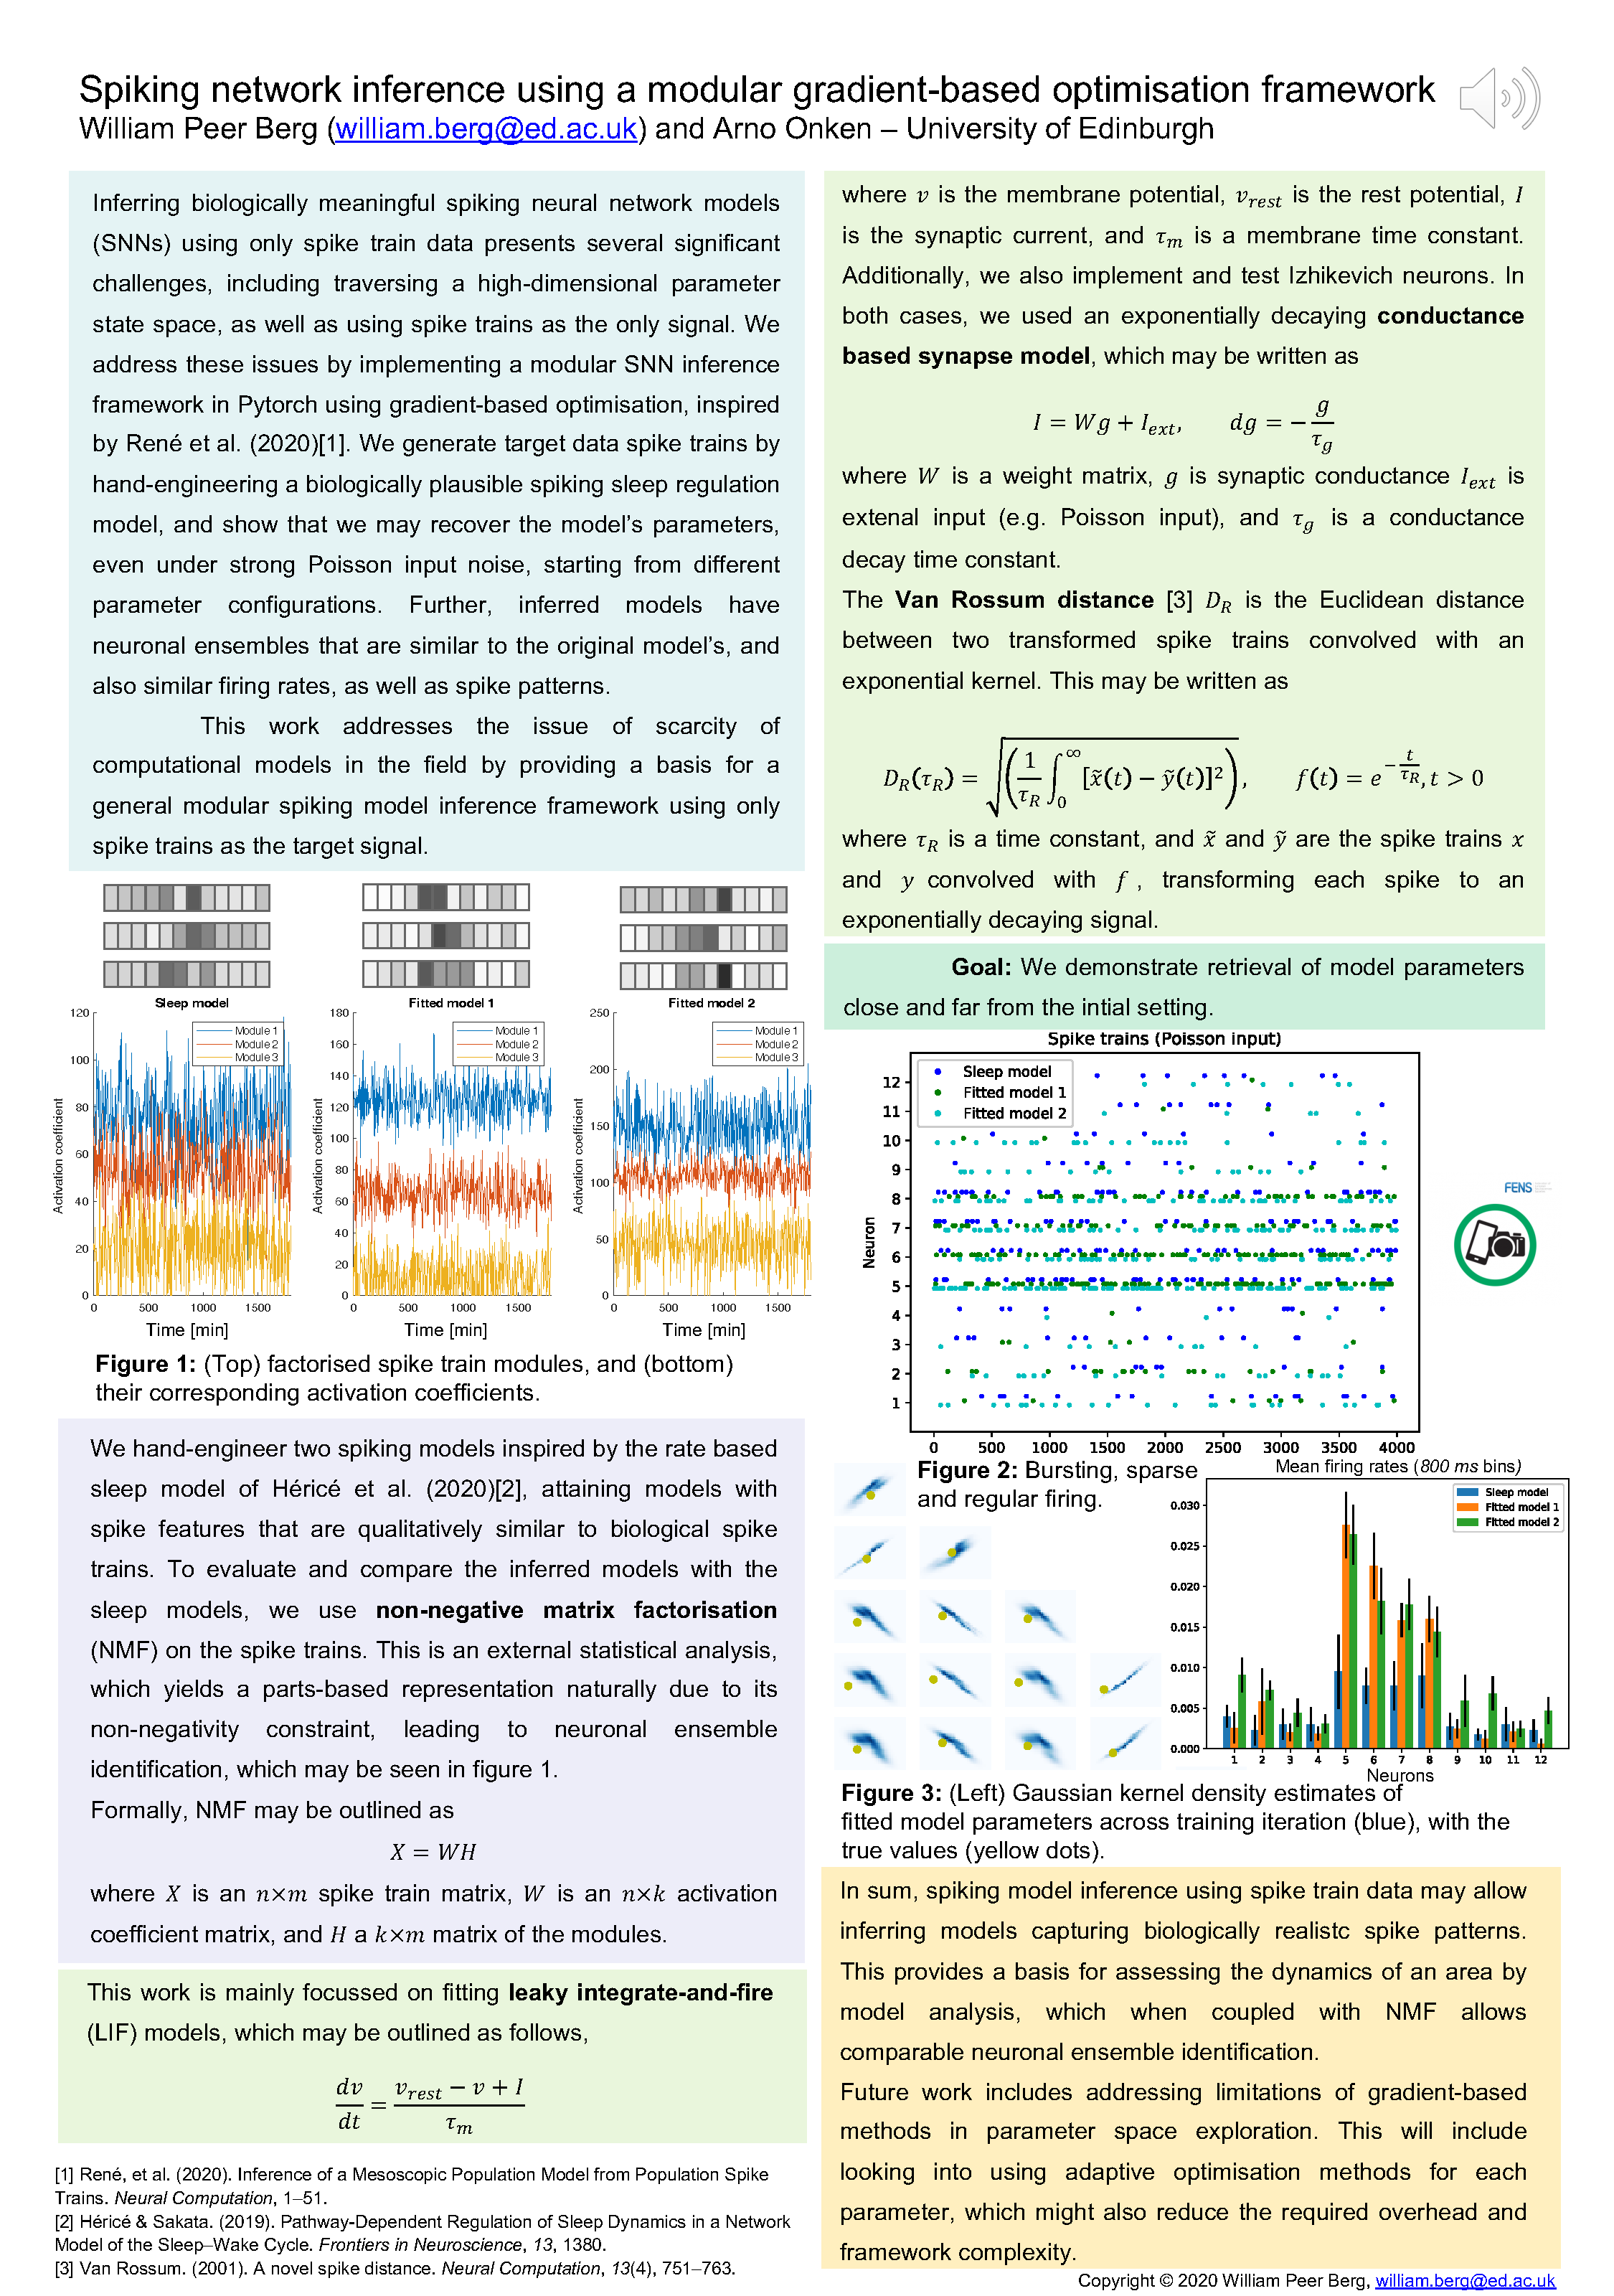
\includepdf[pages=-]{files/FENS-virtual-2020-e-Poster-W-P-Berg-and-A-Onken-Spiking-Network-Inference-Using-Gradient-Based-Optimisation-PORTRAIT-5.pdf}

\section{Report/paper draft: \textit{Parallel spiking neural network parameter inference using gradient based optimization}}
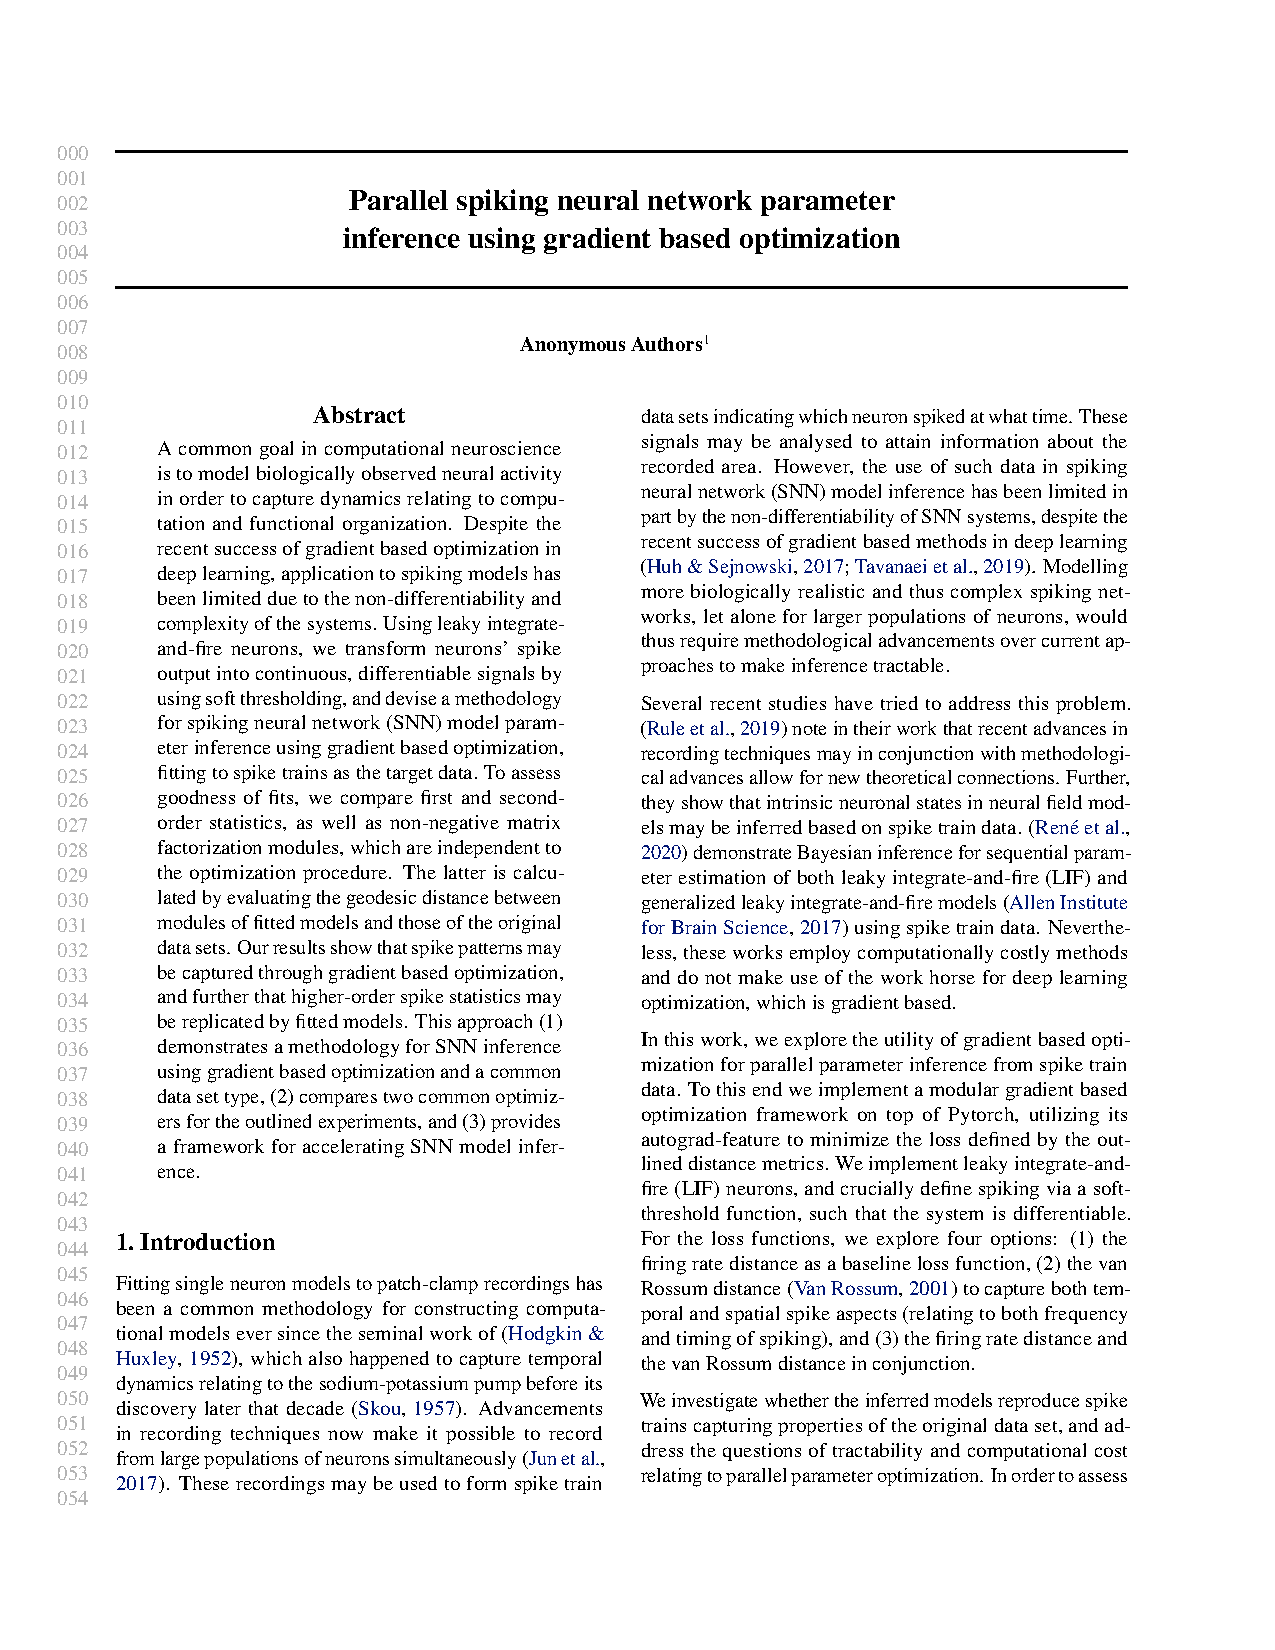
\includepdf[pages=-]{files/icml2021_draft_snn_inference.pdf}

% =======================================================
\chapter{Sleep regulation in the rodent brainstem}

My initial research proposal outlines a research project where the goal is to meet research needs within the field of sleep regulation through computational modelling.
More specifically, the aspiration was to model neurons of the pedunculopontine and laterodorsal tegmental areas within the brainstem during different brain states, based on their neuroanatomy as described, even though scarcely, within the literature, and based on in vivo data from these brain areas \cite{Herice2019c, Tsunematsu2019, Pal2007, Martinez-Gonzalez2011, Fraigne2015}.
Further, an overarching research goal was to be able to capture the emergence of neural ensembles as identified in vivo in the model by using non-negative matrix factorisation (NMF) \cite{Seung1999, Seung2001, Onken2016a}.
Computational modelling and spiking neural network (SNN) inference covers several research needs within the field of sleep research and the synthesis of neuroscience and its computational counterpart in that it addresses model scarcity, as well as a methodology for accelerating modelling by inference through gradient-based optimisation \cite{Herice2019c, Huh2017, Taherkhani2020}.
This was the foundation for sparking my interest in a methodological project in which we seek to automate biologically relevant neural network model inference, and more specifically to research both (1) the current state-of-the-art on SNN inference, and (2) leveraging ML based methods of gradient descent and optimisation for SNN inference \cite{Huh2017, Mostafa2020, Tavanaei2019b, Lee2016}.


\section{Modelling sleep regulation in the brainstem}

Sleep is widespread across different animal species, crucial to mental functioning. However, why we sleep, and how we sleep, remains to be understood. Some models exist that seek to capture the phasic nature of sleep, but mostly at an abstract level. There is as such a need for detailed models in the field, with no current models encompassing direct biological parallels. Addressing the need for modelling in the field, and seeking to illuminate how we sleep, we propose to use a set of recently combined methodologies that allow us to infer the most probable neuron-level spiking models based on only partial information, and partial neuronal recording data. In other words, the methodology allows for incorporating both existing knowledge, and to use spike sorted LFP recordings to infer the most statistically probable distributions of model parameters.

More specifically, using spike sorted data recorded from the mouse brain stem in the pedunculopontine and laterodorsal tegmental (PPT/LDT) areas, we address whether these areas do in fact initiate sleep stages, which has been previously hypothesised and recently debated. 
To address this, we looked at the temporal relationship between future and past state prediction, using linear discriminant analysis (LDA) on derived functional modules using non-negative matrix factorisation (NMF), replicating and extending the work reported by the collaborative lab from whom we have been granted access to the spike data.

Further, we study methodologies for inferring meaningful computational models using spike train data, and how they inferred models may be studied to evaluate the nature of the neurons by drawing upon the biology corresponding to their parameters within the literature.
This algorithmic approach applied to spike train data has, to the best of my knowledge, not been previously explored. This is due to the high dimensional parameter search space, which requires a correspondingly complex approach in order to make computation tractable.
As such, not only could an inferred model be used to address hypotheses such as whether sleep regulation within this area is mediated by an ensemble of cholinergic neurons, but the methodology could further be applied in other domains, using data of the same nature from different brain regions.
The approach requires only partial data - as is always a constraint within neuroscientific recordings. Using a form of Bayesian inference, measures of deviation and confidence may be defined comparatively between synthetic models and data, and the recorded spike trains considered as ‘ground truth’. Probable fits with a fair variance suggest meaningful inferred model parameter distributions. However, model quality metrics depend on the data for which the comparison is computed.

In more detail, the model inference method is based on modelling the probability of spiking for a neuron as a Bernoulli random variable, with the variable modelling spiking in each time bin. We construct time bins for the spike trains such that the probability of spiking in one bin may be approximately dependent only on the previous bin (which might be justified considering its refractory and synaptic time constants). This allows us to formulate the probability of a spike train as a Markov chain, and enables us to estimate population model parameters. Interestingly, the authors found that a better fit for a microscopic model was inferred when first performing gradient descent for a mesoscopic level model, representing each population with average parameters. 
This may be due to that inferring only one average parameter value per population regularises the training procedure by averaging over the parameter space of a microscopic model. 
There are two key points that I would like to communicate associated with that observation; (1) is that the complexity associated with the parameter space of microscopic models might make convergence towards a global optimum unlikely, and (2) that an average parameter might lose values that are of a secondary or tertiary order of importance, despite prominent in the data set, if somewhat conflicting with the final inferred average value. Addressing (2), it might be fruitful to allow for sets of average values for population models, investigating whether this might increase resulting microscopic model performance. Note that inference of the maximum a posteriori for corresponding microscopic models then might increase exponentially, or at least linearly, with the order of increased number of values inferred at the mesoscopic level. However, it might make sense to infer one average per neuron type as the population level, i.e. if it is believed that it contains for instance two sets of neuron types, or functional ensembles, such as inhibitory-excitatory neurons. This has to my knowledge not been attempted within this methodological approach.
Once a mesoscopic model has been attained, it may be used to synthetically generate data for use in the inference of a more detailed neuron-level or microscopic model. By generating synthetic data we may employ the family of Monte-Carlo (MC) methods. In order to accelerate convergence for computational efficiency, Hamiltonian MC is employed. This allows for approximating the full posterior over the most likely parameter distributions for microscopic models.

Statistically, model soundness may be considered in terms of comparison to a validation set stemming from the same experiment, and also across the 7 performed experiments. However, due to the nature of neuroscientific recordings, where there is a significant uncertainty in both the areas targeted with the silicon probes, and not the least due to significant individual differences for neural ensembles, it is unlikely that we can see neuron-level similarities across experiments. However, similarities at a population and functional level may occur if the same areas are recorded.

% Currently, the project is a work in progress, with implementation of the model and a corresponding gradient descent (GD) as well as HMC being in focus. GD may be partially implemented using the Theano library, as well as open-sourced modules, and HMC using the PyMC3 library.
% In order to finalise the implementation, there is a substantial amount of programming required, followed by an ever greater extent of testing, debugging, verification. Finally, when satisfied with the aforementioned, we may proceed to run experiments, analysing the results, and depending on the outcomes pursue further work.



\section{Neuroscience background}

\subsection{Sleep stages}
Three-process switch model. Different timescales may be at play, and constitute the switching-mechanism.
Also, can a meso-model be used in the first step of creation of such a model?

\subsection{PPT/LDT}
PPT/LDT LFP data; most spiking during NREMS
(to consider: Little time spent in NREMS)
Want to primarily look at REMS: disinhibition of monoaminergic LC projections (prerequisite; Timofeev et al. (2017)) (shut off / inhibited in LC by GABA), 

PPT/LDT:
Cholinergic are REMS and wake
GABAergic; REMS, wake, or both
NREM?

Look at single-cell resolution connectivity? (e.g. Martinez-Gonzalez, Mena-Segovia)

Complex circuitry means a myriad of ppt/ldt inputs, some of which are poorly understood.
Could these somehow be reverse-engineered given the state and neural activity, classifying the neurons into types, which can tell us something about the pathways involved, and whether they’re “ON” or “OFF”?
Simple state-driven input as on/off per state to the ensembles should tell us something about each ensemble and its state-preference? If so, these can be identified, parameters compared and fixed, and then we could try to reconstruct the projections - perhaps using the model of Herice et al. (2018)


\section{Analysis of data}
Data from PPT/LDT area/brainstem. Evaluation and assessment through (rigorous) analysis and classification/prediction of brain state. Shows four well-qualified experiments for further analysis and bridging using the mesoscopic modelling approach.
Provides a solid bridge from the domain of experimental data to generating data using a simulated model that is derived from a good data foundation that we know is well-aligned with brain state.

% Idea: “ultradian” process for synchronous/asynchronous activity -> nREM/REM, also should give rise to qualities during wakefulness (such as better brainstorming/creativity, or some types of productivity in “phases”/stages)

% Idea: Cell types and model parameters that may be used in type classification from fitting data to GLIF models is lacking for the mouse brainstem in the Allen Brain project database.

Replicated results of \cite{Tsunematsu2019}, finding that NMF ACs were more indicative of future brain state than HPC signals, which was a novel finding presented in the original work.
This also means that the data should contain information that if captured in a model may illuminate the functional dynamics associated with sleep regulation in the area (PPT/LDT).

In order to test whether ...
% See first year(?) review
Two-sided LDA - no improved results.
However, single-neuron signals slightly better predictors - suggesting both that there was some information lost in factorisation, but also that the ensembles were very good representations of functional units, as argued in the original paper.


\section{Inference}

\subsection{GBO}

\subsection{ABC}

\section{Conclusion}

% =======================================================
\chapter{BONUS: Exact models with continuous spike signals}

Non-leaky integrate-and-fire (NLIF) model with subthreshold continuous spike signals defined to sum to 1 inside of an active zone \cite{Huh2017}.
% With NIF neurons, one could analytically show/solve the systems and show where noise would render the loss function useless. However, unsure how to test this for spike output task. Could we use (Mostafa, 2018) combined with (Huh \& Sejnowski, 2017)? Or at least the latter?

\section{Gated sub-threshold spike-signal model}

\section{Study: \textit{NLIF for exact gradient based model inference}}

\subsection{NLIF definition}

\subsection{Tasks}

\subsection{Synapse types}

\subsection{Discussion}

analog output versus discrete pulses and latent internal states (??)
research has been impeded by lack of supervised learning algorithms
they present differentiable formulation of SNNs, with exact gradient calculation
simple tasks
rate-based models fail to describe fast dynamics of spike-based computation
difficult to optimise discrete, binary all-or-none signals
other methods circumvent non-differentiability

"Note that the gradient calculation procedure involves multiplication between the presynaptic input source and the postsynaptic adjoint state pv, which is driven by the g ˙ps term: i.e. the product of postsynaptic spike activity and temporal difference of error. This is analogous to reward-modulated spike-time dependent plasticity (STDP) [17]."



% =====================================================
\chapter{(Discussion) Working title: Why the brain does not do backpropagation}

Receptive fields very robust, but continuous perturbation results in changes, also in higher visual areas
Individual differences
The brain is “born with too many neurons” - naturally does pruning
“Some neurons and parameters are highly important, whereas others aren’t” - Fisher information spans an ellipse in parameter-space(?), can see that some aren’t that important
Q: Can we compute the Fisher information locally? Essentially, yes. Parameter importance. Can also go further and do mean field approximation. ML does something like this. Local heuristics can be used efficiently to remove many parameters in network without “interference”. Turns out many of related neurons may be pruned away too.
Brain neurons highly recurrently connected.
Q: How does the brain do things?
Synaptic conn in brain constrains what patterns are visible to neurons
Brain is a dyn cyst
Can compute manifolds in which the activity lives and moves
Functioning: “Carried out by movements along manifolds”
Activity is modulated by incoming activity, which manipulate manifolds


If the structure that allows acquisition of new knowledge, as well as new heuristics, is successfully implemented, the ever-changing heuristics may lead to an autonomous agent. 
However, successfully implementing the aforementioned is an engineering challenge we have yet to overcome. It is difficult to predict what such an algorithm would need to contain, as most applications of DNNs are very domain specific, and extremely or fully prone to catastrophic forgetting when trained on a new data set.
There is still a fundamental gap between general knowledge acquisition and the specialised kind we see within ML.


“Computationally, we now know that optimization of trajectories gives rise to elegant solutions for very complex motor tasks (Harris and Wolpert, 1998; Todorov and Jordan, 2002; Mordatch et al., 2012). We suggest that cost function optimization occurs much more generally in shaping the internal representations and processes used by the brain. Importantly, we also suggest that this requires the brain to have mechanisms for efficient credit assignment in multilayer and recurrent networks.” - Marblestone et al. (2016). Frontiers in Computational Neuroscience
And it doesn’t matter what specific configuration a network reaches, as long as it reaches “the bottom of the loss curve”, i.e. finds a good/satisfactory solution. → Optimal is any configuration solving the task at hand, and optimal is plural, and diverse. Optimal can be a frontier in high-dimensional space. In Bayesian inference Macke argued we may be able to trace this front by drawing shapes between samples forming probable combinations in parameter-space.

Can we say something about this Pareto-front with GD?
When sampling from full posterior dist from a SBI posterior we get realistic data - when independently sampling from marginals we get unrealistic data. Flaw in model, and in assuming parameter independence.

Both of these methodologies get at a reasonable frontier - however, learning in itself in the structures is something different, remaining a mystery.


If only the temporal unfolding of spike events was done according to linear transformations, or in a ...
It may be argued that under similar conditions, we may detect things such as spike correlations and phase-locking, which may indicate a clear function of the timing of spiking in information processing - however, it is difficult to design a loss metric that would well capture this in a differentiable manner.
By correlation and number of mutations of the ordered spike train set, we can get closer to this - but such a metric would not be differentiable, nor would even such a metric be able to precisely measure whether one network is functionally equivalent to another.
Part of the difficulty stems from that (1) there are multiple configurations which can produce similar spike patterns, and thus we may hypothesise that there is no "ground-truth" optimal solution per se, and (2) due to the multiple factors of stochasticity we cannot operate with precise spike train comparisons. These two points result in that currently the way of going about to analyse biologically realistic models are closer to the way we analyse recordings from the biological brain. As such, a bridge between inference methodologies such as the ones successfully employed in ML, and the field of computational modelling is needed.


\bibliographystyle{plain}
\bibliography{references}

%% You can include appendices like this:
% \appendix
\appendix\label{appendix:sample_GLM_code}
\title{Sample GLM code}

% 
% \chapter{First appendix}
% 
% \section{First section}
% 
% Markers do not have to consider appendices. Make sure that your contributions
% are made clear in the main body of the dissertation (within the page limit).
% TODO: What is the page limit?

\end{document}
